\documentclass[titlepage, a4paper]{article}
\usepackage[utf8]{inputenc}
\usepackage{amsmath}
\usepackage{amssymb}
\usepackage{amsthm}
\usepackage{hyperref}
\usepackage{cleveref}
\usepackage{geometry}
\usepackage{enumerate}
\usepackage{mathtools}
\usepackage{tikz-cd}
\usepackage{tikz}
\usepackage{todonotes}
\usetikzlibrary{fit,arrows,calc,positioning}
\usepackage[backend = biber,style=alphabetic]{biblatex}
\addbibresource{references.bib}
\usepackage[parfill]{parskip}
\usepackage{appendix}
\usepackage[nottoc,numbib]{tocbibind}

\makeatletter
\def\input@path{{../Bewijzen/}}

\makeatother



\author{Lucas Levrouw \and Michaël Maex \and Tomas Reunbrouck \and Supervisor: Gabor Szabo}

\title{Kaplansky's Direct Finiteness Conjecture and Sofic Groups}

\date{\today}

\newcommand{\N}{\mathbb{N}}
\newcommand{\Z}{\mathbb{Z}}
\newcommand{\Q}{\mathbb{Q}}
\newcommand{\R}{\mathbb{R}}
\newcommand{\C}{\mathbb{C}}
\newcommand{\F}{\mathbb{F}}

\newcommand{\card}[1]{\left| #1 \right|}
\newcommand{\inclusion}[1]{\xhookrightarrow{#1}}
\newcommand{\surjection}[1]{\xtwoheadrightarrow{#1}}
\newcommand{\id}{\mathrm{id}}
\DeclareMathOperator{\sym}{Sym}
\DeclareMathOperator{\im}{im}
\DeclareMathOperator{\red}{red}



\newtheorem{theorem}{Theorem}[section]
\newtheorem{proposition}[theorem]{Proposition}
\newtheorem{lemma}[theorem]{Lemma}
\newtheorem{conjecture}[theorem]{Conjecture}
\newtheorem{corollary}[theorem]{Corollary}
\newtheorem{property}[theorem]{Property}
\theoremstyle{definition}
\newtheorem{definition}[theorem]{Definition}
\theoremstyle{remark}
\newtheorem{example}[theorem]{Example}
\newtheorem{remark}[theorem]{Remark}

\usepackage{import}
\usepackage{xifthen}
\usepackage{pdfpages}
\usepackage{transparent}

\newcommand{\incfig}[1]{%
    \def\svgwidth{.5\columnwidth}
    \import{../Figuren/}{#1.pdf_tex}
}

\newcommand{\nocontentsline}[3]{}
\newcommand{\tocless}[2]{\bgroup\let\addcontentsline=\nocontentsline#1{#2}\egroup}

\makeatletter
\newcommand{\customlabel}[2]{% \protected@write @auxout {}{\string \newlabel {#1}{{#2}{\thepage}{#2}{#1}{}} }% 
\hypertarget{#1}{}}

\makeatother

\begin{document}
\pagenumbering{Alph}
    \maketitle
\pagenumbering{arabic}
\tableofcontents
\pagebreak

\section{Introduction}\label{sec:intro}

\subsection*{The Lay of the Land}

This report discusses a conjecture of Kaplansky which states that any group ring $\mathbb{K}[G]$ with $\mathbb{K}$ a field is directly finite. That is, the left-invertibility of elements implies their right-invertibility. For general groups and fields, this conjecture sofar has remaing open. It has been resolved, however, for specific cases, in particular the case in which the group $G$ is sofic, which means that in some sense $G$ can be approximated well with finite groups. Some cases require the assumption of another conjecture. For example, when we talk about finite fields $\mathbb{K}$ we have a positive result for Kaplansky’s conjecture for surjunctive groups (definition in section \ref{sec:surjunctivity}). The class of surjunctive groups is very large and possibly contains all countable groups. Therefore, if we were to have that all countable groups are surjunctive, this positively resolves Kaplansky's conjecture for finite fields and countable groups.
The assumption that all countable groups are surjunctive is known as the conjecture of Gottschalk and will be discussed in detail.

\subsection*{Historical Context}

We can trace the origins of the concepts we shall discuss back to the research by John von Neumann throughout the 20th century. First, he introduced the notion of amenable groups in the context of the Banach-Tarski Paradox. It was meant as a generalisation of commutative groups on the one hand and various versions of finite groups on the other. Secondly, he lay the foundations of the study of so-called ‘cellular automata’. What a cellular automaton is, can be explained the following way. Take a set $A$ (finite or infinite), of which we call the elements ‘states’, and a ‘universe’ of ‘cells’, being a countable group $G$. Now $A^G$ (the set of maps $G \to A$) is the set of configurations. The automaton, then, is a map from $A^G$ to itself, satisfying the property that the state of a specific cell in the image is determined by the initial states of the cells in a bounded neighbourhood of this cell \cite{vonNeumann_1966} .\\
\\
These two concepts may, at first glance, seem completely unrelated. The connection becomes clear, however, when considering the question of surjectivity of these maps on the configuration space. Surjectivity in this context is, intuitively, the property that any configuration can be reached as a result from some other configuration. A configuration that can not be produced because it is not in the image of the (non-surjective) automaton is called a ‘Garden of Eden’. Importantly, such a Garden of Eden always contains a so-called ‘orphan’ which is a finite subset which cannot be produced (a finite Garden of Eden, as it were). The Garden of Eden Theorem states that a configuration is a Garden of Eden if and only if it contains such an orphan. From this theorem it follows that the injectivity of the automaton implies its surjectivity. However, the validity of this theorem has only been proven for amenable groups.
Now, groups $G$ for which it is the case that injectivity of an automaton using any finite alphabet implies surjectivity of that automaton are the afore mentioned surjunctive groups. This, then, brought research eventually to sofic groups, as this is the largest known class of groups of which all members are known to be surjunctive \cite{ceccherini-silberstein_coornaert_2010}.  
\todo{Hoe werkt de garden of eden theorem $\implies$ surjunctive?}

\subsection*{Goal of this Report}

We shall mainly focus on the following two concepts: soficity and surjunctivity. First we shall discuss what it means for a group to be sofic. It is a very large class of groups. In fact, there exist no known examples of non-sofic groups \cite[introduction]{weiss_2000}. This will be illustrated by proving soficity for a few large classes of groups. Furthermore, we shall discuss its connections to other important concepts and group properties such as amenability. Secondly, this report will cover surjunctivity which is related to soficity but will be used to discuss the connection between the conjectures of Kaplansky and Gottschalk. Specifically, it is known that all sofic groups are surjunctive as well.
Finally, we will discuss Kaplansky's conjecture in the context of finite fields. More precisely we will give the details of a proof that the group ring a surjunctive group and finite field is directly finite. \Cref{fig:dependency_graph} shows how how the different concepts in this report relate to each other.


\begin{figure}[h]
	\centering
\begin{tikzcd}
	\text{$G$ is Residually Finite} \arrow[dr, Rightarrow] \\
	& \text{$G$ is Sofic} \arrow[r, Rightarrow] & \text{$G$ is Surjunctive} \arrow[r, Rightarrow] & \text{$\F_{p^{k}}[G]$ is Directly Finite}\\
\text{$G$ is Amenable} \arrow[ur, Rightarrow]
\end{tikzcd}
\caption{A dependency graph of the relevant theorems/properties. }
\label{fig:dependency_graph}
\end{figure}
\section{Group Rings}\label{sec:group_rings} 
% Szabo's comment: Is there a reason you single out these fields here?

The setting of Kaplansky's direct finiteness conjecture is about so-called group rings. These are defined as follows


\begin{definition}\label{def:group_ring}
	Let $\mathbb K$ be a field and $G$ be a group. The \textbf{group ring} $\mathbb K[G]$ is the set of formal linear combinations
    \[
        \sum_{g \in G} \lambda_g g,
    \]
    where $\lambda_g \in \mathbb K$ for all $g \in G$ and only finitely many $\lambda_g$ are nonzero. The operations $+$ and $\cdot$ are defined by
    \begin{align*}
        \sum_{g \in G} \lambda_g g + \sum_{g \in G} \mu_g g
        &= \sum_{g \in G} (\lambda_g+\mu_g) g \\
        \left(\sum_{g \in G} \lambda_g g \right) \cdot \left(\sum_{g \in G} \mu_g g \right)
        &= \sum_{g \in G} \left( \sum_{h \in G} \lambda_{h} \mu_{h^{-1}g} \right) g.
        %\sum_{g \in G} \left( \sum_{\substack{g_1, g_2 \in G \\ g_1 g_2 = g}} \lambda_{g_1} \mu_{g_2} \right) g.
    \end{align*}
\end{definition}


\begin{proposition}
    Let $\mathbb K$ be a field and $G$ a group. Then $\mathbb K[G]$ is a unital ring.
\end{proposition}
The proof of this theorem is no more than checking the group axioms one by one. For completeness you can find it in appendix \hyperlink{sec:proof_groupring}{A}.

\begin{remark}
	A group ring in general is not commutative. In fact $\mathbb{K}[G]$ is commutative if and only if $G$ is a abelian group. So we will have to be careful when dealing with these rings. 
\end{remark}

We can now state Kaplansky's conjecture by the example of the introduction in \cite{elek_szabo_2003}.

\begin{conjecture}[Kaplansky]
	Let $\mathbb K$ be a finite field and $G$ a group. Then $\mathbb K[G]$ is directly finite i.e. for all $a, b \in \mathbb K[G]$, the equation $ab=1$ implies $ba=1$.
\end{conjecture}

To put it shortly, Kaplansky's conjecture states that for all elements in the group ring, left-invertible implies right-invertible. If we work over a finite field $\F$ and $G$ is a finite group, it can quite easily be proven that $\F[G]$ is directly finite.

\begin{theorem}
    Let $\F$ be a finite field and $G$ be a finite group. Then $\F[G]$ is directly finite. 
\end{theorem}
\begin{proof}
    Let $a, b \in \mathbb F[G]$ and suppose $ab=1$. Now consider the map
    \[
        \phi: \mathbb F[G] \to \mathbb F[G]: x \mapsto x a
    \]
    This map is injective. To see this, let $x, y \in \mathbb F[G]$ such that $xa=ya$. Multiply on the right with $b$ and use the associativity to conclude $x=y$.
    But since $\mathbb F[G]$ is a finite set, the map must also be surjective. Therefore there exists an $x \in \mathbb F[G]$ such that $x a = 1$. Furthermore, $x = xab = b$. So we have $x = b$.
\end{proof}

Note how the argument hinges on the fact that the map $\phi$ is guaranteed to be surjective by the finiteness of $\mathbb F$ and $G$. In what follows we will define several ``finiteness'' properties of groups and try to generalise the proof above under weaker assumptions.

\section{Sofic Groups}\label{sec:sofic_group}

\subsection{Definition and Motivation}

In this section we will introduce the concept of a \emph{sofic group}. A sofic group is a group that is ``well approximated'' by a finite permutation group. Recall that every finite group is isomorphic to the subgroup of a permutation group.
% Szabo: definitely no. What do you mean by finite permutation groups?

To define this, we will need a way to measure a distance between permutations. It is quite natural to define the distance between two permutation as the fraction of elements on which they differ \cite[subsection 2.1]{capraro_lupini_2015}.

\begin{definition}
    The \textbf{Hamming distance} on $\sym(n)$ is defined by
    \[
        d_{\sym(n)}(\sigma, \tau) = \frac 1 n \card{\{k \in \{1, 2, \dots,n\} \mid \sigma(k) \neq \tau(k)\}}, 
    \]
    for every $\sigma, \tau \in \sym(n)$.
\end{definition}

It is easy to show that $d_{\sym(n)}$ is a metric.
We might call a group well-approximated by finite permutation groups if there exists a sequence of ``approximate morphisms''
$(\Phi_i: G \to \sym(d_i))_{i \in \N}$ which mimic the group structure of $G$ better and better in $\sym(d_i)$ as $i$ tends to infinity. %akward phrasing?
For that, we first of all want that $d_{\sym(d_i)}(\Phi_i(g) \circ \Phi_i(h), \Phi_i(gh))$ converges to zero, for every $g$ and $h$ in $G$. Additionaly, we want that in the limit these maps have a sort of injectivity property. Therefore we will require all elements of $G$ except the identity element to converge out of the kernel of these maps. We add the following condition \footnote{One might wonder why we do not require that every $g \neq 0$ converges to some fixed strictly positive number $r(g)$ instead. In fact one can show that if that is the case, one can construct another sequence of maps $\Phi_i' : G \to \sym{d_i'}$ such that $d_{\sym(d_i')}(\id, \Phi_i'(g))$ converges to $1$ for every $g$ (\cite{capraro_lupini_2015}, definition 2.2.2) }
\[
\lim_{i \to \infty} d_{\sym(d_i)}(\id,\Phi(g)) = \begin{cases}  0 & \text{if } g = 1_G \\
                                        1 & \text{otherwise,}
                                        \end{cases}
\]
where $1_G$ denotes the identity element of $G$ and $\id$ is the identity permutation.
\\

We can now state the definiton of a sofic group based on \cite[section 1]{kerr_li_2010}.

\begin{definition}{}\label{def:Sofic}
        Let $G$ be a countable group. We say that $G$ is \textbf{sofic} if there exists a sequence of natural numbers $(d_i)_{i \in \N}$ with associated maps $\Phi_i : G \to \sym(d_i)$ such that for all $g, h \in G$:
        \begin{enumerate}[(i)]
            \item $ \displaystyle \lim_{i \to \infty} d_{\sym(d_i)}(\Phi_i(g) \circ \Phi_i(h), \Phi_i(gh)) = 0$
            \item $ \displaystyle \lim_{i \to \infty} d_{\sym(d_i)}(\id,\Phi(g_i)) = \begin{cases}  0 & \text{if } g = 1_G \\
                                                                                    1 & \text{otherwise,}
                                                                                    \end{cases}$
        \end{enumerate}
        %where $\delta_{e,g}$ is $1$ if $g = e$ and $0$ otherwise. (this is unnecessary as we don't use delta in the definition; that is why szabo wrote '?', not because of the 'sofic approximation'. Yours sincerely, Tomas
    \end{definition}

    We will call such a family of maps $\left(\Phi_i : G \to \sym(d_i) \right)_{i \in \N}$ 
    a \emph{sofic approximation sequence} for $G$. It is unkown if every group is sofic.

    We can also reformulate the two conditions in a form more suitable for calculations.
     \begin{lemma}
        Let $G$ be a countable group. Then $G$ is sofic if and only if there exists a sequence of natural numbers $(d_i)_{i \in \N}$ with associated maps $\Phi_i : G \to \sym(d_i)$ such that for all $g, h \in G$:
        \begin{enumerate}[(i)]
            \item $\displaystyle \lim_{i\to \infty} \frac{1}{d_i} \card{\big\{k \in \{1, \dots, d_i\} \mid (\Phi_i(g) \circ \Phi_i(h))(k) = \Phi_i(gh) (k) \big\}} = 1$
            \item $\displaystyle \lim_{i\to \infty} \frac{1}{d_i}  \card{\big\{k \in \{1, \dots, d_i\} \mid \Phi_i(g)(k) = k \big\}} = \begin{cases}  1 & \text{if } g = e \\
                                                                                    0 & \text{otherwise.}
                                                                                    \end{cases}$
        \end{enumerate}

    \end{lemma}


    \subsection{Examples of Sofic Groups}
    The Sofic groups are a very large class of groups. 
    In fact there are no known examples of non-sofic groups \cite[Introduction]{weiss_2000}. 
    Here we will list some groups that we know are sofic.
    
    
    \begin{example}\label{ex:finite_group_sofic}
    Consider a finite group $G$. Look at the map $\phi: G \to \sym(G): g \mapsto s_g$, where $s_g$ is defined by $s_g(h) = gh$. Clearly, $\phi$ is a homomorphism. Now we can choose $d_i = \card G$ and $\Phi_i = \phi$ for all $i \in \N$. Here we have identified $\sym(G)$ with $\sym(d_i)$. The first condition is satisfied since $\phi$ is a morphism. The second condition follows from the fact that $s_g(h) = gh = h$ if and only if $g$ is the identity.
     Hence every finite group is sofic.
    \end{example}

    % Example: Z

	\begin{example}\label{ex:Z}
	Consider the group $\Z$. Take the sequence of maps $\Phi_{i}: G \to \sym(i): g \mapsto \Phi_{i}(g)$ where $\Phi_{i}(g)$ is defined as the map such that for any $k \in \{1,\dots,i\}$ : $ \Phi_{i}(g)(k) = (g+k) \mod i$. The first condition of soficity is satisfied as for any $i \in \N, g,h \in \Z, k \in \{1,\dots, i\}$ it can be said that 
	\begin{align*}
	(\Phi_{i}(g) \circ \Phi_{i}(h))(k) &= (g+h+k)\mod i \\
	&= \Phi_{i}(g+h)(k)
\end{align*}		
Now for the second condition. It is clear that for any $i \in \N, k \in \{1,\dots, i\}$ : $\Phi_{i}(0)(k) = k$. Now take any $g \neq 0$ and consider $\Phi_{i}(g)$. For any $k \in \{1,\dots,i\}$ it is perfectly possible that $\Phi_{i}(g)(k) = k$. However this is not the case as soon as $i > |g|$. In that case, we have that $|(k+g)-k| < i$, from which it follows that $(k+g) \neq k \mod i$. Thus we have that $(k+g) \neq k \mod i$. Therefore, $\Phi_{i}(g)(k) \neq k$, proving the second condition. 
	\end{example}
    % Example: Direct product of sofic groups is sofic. 

    \begin{example}\label{ex:direct_product_sofic}
        The direct product of two sofic groups is again sofic. Consider two sofic groups $G$ and $H$. Let $(\phi_i: G \to \sym(n_i))_{i \in \N}$ and $(\psi_i: G \to \sym(m_i))_{i \in \N}$ be sofic approximation sequences for $G$ resp. $H$. Consider in this example $n_i = \{0, \dots, n_i-1\}$ and $m_i=\{0, \dots, m_i-1\}$. For every $i\in \mathbb N$ we can define $\Psi_i: G \times H \to \sym(n_i \times m_i)$ by $\Psi_i(g,h)(k, l) = (\psi_i(g)(k), \phi_i(h)(l)) \in \sym(n_i \times m_i)$.
        Then we have
        \begin{multline*}
        	\frac{1}{n_i m_i} \card{\big\{(k,l) \in n_i \times m_i \mid (\Phi_i(g,h) \circ \Phi_i(x,y))(k,l) = \Phi_i(gx,hy)(k,l) \big\}} \\
        	= \frac{1}{n_i m_i} \card{\big\{(k,l) \in n_i \times m_i \mid (\phi_i(g) \circ \phi_i(x))(k) = \phi_i(gx)(k) \text{ and } (\psi_i(h) \circ \psi_i(y))(l) = \psi_i(hy)(l)\big\}} \\
        	= \frac{1}{n_i m_i} \card{\big\{ k \in n_i \mid (\phi_i(g) \circ \phi_i(x))(k) = \phi_i(gx)(k)\big\}} \cdot \card{\big\{l \in  m_i \mid (\psi_i(h) \circ \psi_i(y))(l) = \psi_i(hy)(l)\big\}},
        \end{multline*}
        and this converges to $1$ because $(\phi_i)_{i \in \N}$ and $(\psi_i)_{i \in \N}$ are sofic approximation sequences. Similarly,
        \begin{multline*}
        	\frac{1}{n_i m_i} \card{\big\{(k,l) \in n_i \times m_i \mid (\Phi_i(g,h)(k,l) = (k,l) \big\}} \\
        	= \frac{1}{n_i m_i} \card{\big\{(k,l) \in n_i \times m_i \mid \phi_i(g)(k) = k \text{ and } \psi_i(h)(l) = l\big\}} \\
        	= \frac{1}{n_i m_i} \card{\big\{ k \in n_i \mid \phi_i(g)(k) = k \big\}} \cdot \card{\big\{l \in  m_i \mid \psi_i(h)(l) = l\big\}},
        \end{multline*}

        and this converges to $1$ if $(g,h)=(1_G, 1_H)$ and to $0$ otherwise. We thus have constructed a sofic approximation sequence $(\Phi_i: G \times H \to \sym(n_i m_i))_{i \in \mathbb N}$, where we now have identified $\sym(n_i \times m_i)$ with $\sym(n_i m_i)$.


 %        Now consider $\Phi_i : G \times H \to \sym(d_i+e_i)$ for every $i \in \N$, where $\Phi_i(g, h) \in \sym(d_i+e_i)$ is defined by
 %        \[
 %            \Phi_i(g,h)(k) = \begin{cases} \phi_i(g)(k) & \text{if } 1 \leq k \leq d_i \\
 %            \psi_i(h)(k)+d_i & \text{if } d_i + 1 \leq k \leq e_i
 %            \end{cases}.
 %        \]
 %        It is not hard to show that $(\Phi_i)_{i \in \N}$ is a sofic approximation sequence for $G \times H$. % Write out proof
	% Hence finite direct products conserve the soficity property. \todo{Write out proof}
    \end{example}

    In the next sections we will introduce two classes of groups that are sofic, \emph{amenable groups} and \emph{residually finite groups}. Since it is often easier to check these properties than to work with the definition of soficity, this will allow us to give some more examples. 
    Some notable examples are 
    \begin{itemize}
	    \item countable abelian groups (\cref{thm:countable_abelian_folner})
	    \item countable solvable groups (\cref{thm:countable_solvable_amenable})
	    \item finitely generated free groups (\cref{ex:free_group_residually_finite})
    \end{itemize}
    

    \section{Amenability} \label{sec:amenable}

	\subsection{Definition and Examples}

    Amenable groups are a large class of groups. 
    Many equivalent definitions exist. 
    An extensive study of amenable groups goes beyond the scope of this project. Hence we will not give multiple definitions and prove equivalence nor will we provide proofs for every property of amenable groups.

    For our purposes we will only define amenability for countable groups and take the Følner criterion as definition. In \cite[subsection 4.1]{kerr_li_ergodic_theory} an alternative definition is given, and it is proven that this is equivalent to the Følner criterion, as formulated below.
	
    % Lucas: Ik heb geprobeerd alle sporen van `conditie 1' uit te wissen maar misschien moeten jullie ook nog eens kijken of ik niks vergeten ben
    \begin{definition}\label{def:folner} 
	    Let $G$ be a countable group. We say that $G$ satisfies the \textbf{Følner criterion} if there exists a sequence of finite subsets (not necessarily subgroups) $F_1, F_2, \dots \subset G$ such that for all $g \in G$ 
        \[
        \lim_{i\to \infty} \frac{\card{gF_i \triangle F_i}}{\card{F_i}} = 0,
        \]
        where $\triangle$ denotes the symmetric difference.
    \end{definition}
    %\item for every $g \in G$ there exists an $N \in \N$ such that for all $n > N: x \in F_n$
    \Cref{fig:folner} gives a visual intuition for this notion. 
    If a countable group statisfies the Følner condition, we will call the group \emph{amenable}.\footnote{One can also define amenability also for uncountable groups. In that case however, it is defined differently and the Følner criterion is not equivalent to the amenability.}\todo{reference for the footnote} 

\begin{figure}[ht]
    \centering
    \incfig{folner}
    \caption{An illustration of the Følner criterion. The limit means that the gray part will become very small compared to  $F_n$ itself as $n$ gets large.}
    \label{fig:folner}
\end{figure}

By the following lemma, we can not only exploit this for individual elements, but also for finite subsets.
\todo[color=green]{Moet dit lemma naar achter?}
\begin{lemma}\label{lem:folner_finite_subset}
    Let $F_i$ be a Følner sequence. Then for every finite subset $B \subset G$ it holds that  \[
    \lim_{i \to \infty} \frac{\card{BF_i \triangle F_i}}{\card{F_i}} = 0    
    .\] 
\end{lemma}
\begin{proof}
    Suppose that $B = \{b_1, b_2, \ldots, b_r\} $. 
    Have a look at the following calculation:
    \begin{align*}
	    \lim_{n \to \infty} \frac{\card{BF_n \triangle F_n}}{\card{F_n}} &= \lim_{n \to \infty} \frac{\card{BF_n \setminus F_n} + \card{F_n \setminus BF_n}}{\card{F_n}}  \\
									 &= \lim_{n \to \infty}  \frac{\card{\bigcup_{i = 1}^{k} (b_i F_n \setminus F_n)}+ \card{F_n \setminus BF_n}}{\card{F_n}} \\
									 &\le \lim_{n \to \infty} \frac{\sum_{i-1}^{k} \card{b_i F_n \setminus F_n} +  \card{F_n \setminus b_1 F_n}}{\card{F_n}} \\
                                         &\le \lim_{n \to \infty} \sum_{i = 1}^{k} \frac{\card{b_iF_n \triangle F_n}}{\card{F_n}} = 0.  \\
    .\end{align*}
\end{proof}

\begin{example}\label{ex:finite_group_folner}
    Every finite group trivially satisfies the Følner condition. Indeed, we can take $F_i = G$ for every $i \in \N$. Note that $gG \triangle G = G \triangle G = \emptyset$. Hence $\card{gF_i\triangle F_i} = 0$ for all $i \in \N$.
\end{example}

\begin{example}\label{ex:integers_folner}
    The group of integers $\Z$ is also amenable. Let $F_i = \{-i, -i+1, \dots, i-1, i\}$ for every $i \in \N$ and let $k$ be an arbitrary integer. Then
    \[
        \frac{\card{(k + F_i) \triangle F_i}}{\card{F_i}}
        = \frac{\card{\{k-i, k-i+1, \dots, k+i-1, k+i\}\triangle \{-i, -i+1, \dots, i-1, i\}}}{2i+1}
        \leq \frac{2|k|}{2i+1},
    \]
    and this converges to zero as $i \to \infty$.
\end{example}

\begin{example}
	Counterexamples are at least as insightful as examples. 
	The free group $F_n = \left<x_1, x_2, \ldots, x_n \right>, n \ge 2$ is not amenable. % You should first of all properly define what the free group is
	For those not familiar with the free group, a brief introduction is given in appendix \hyperlink{sec:intro_free_group}{B}.
	To prove this we will have to show that there does not exist a Følner sequence.
	We will prove that for every non-empty finite subset $H \subset F_n$ it holds that \[
		\card{\bigcup_{i = 1}^{n} x_iH \cup x_i^{-1}H} \ge (2n-1) \card{H}
	.\] 
	We can prove this using induction on the size of $H$. 
	\begin{description}
		\item[$\card{H} = 1$:] Then $H = \{g\}$. 
			Hence the left hand side set is $\{x_1g, x_1^{-1}, x_2g, x_2^{-1}g, \ldots, x_ng, x_n^{-1}g\} $, which has cardinality $2n$. 
		\item[$\card{H} > 1$:] 
			Let $ h \in H$ be an element that has maximum number of letters in reduced form.
			Consider the set $H' = H\setminus \{h\} $. 
			By the induction hypothesis it holds that 
			\[	
				\card{\bigcup_{i = 1}^{n} x_iH' \cup x_i^{-1}H'} \ge (2n-1) \card{H'}
			.\] 
			For at least $2n-1$ elements of $\{x_1,x_1^{-1},x_2,x_2^{-1},\ldots, x_n, x_n^{-1}\} $ the words $x_ih$ or  $x_i^{-1}h$ have more letters in reduced form than $h$. Let $\Delta = \{ h_1, h_2, \ldots, h_n\} $ be that set.  
			As multiplying by one generator changes the number of letters by $\pm 1$, we see that elements of $\Delta$ are not of the form $x_ih'$ or $x_i^{-1}h'$ for some generator $x_i$ and $h' \in H$. 
			Hence \[
				\card{\bigcup_{i = 1}^{n} x_iH \cup x_i^{-1}H}  \ge \card{\bigcup_{i = 1}^{n} x_iH' \cup x_i^{-1}H'} + 2n-1
 			.\]
			So \[
				\card{\bigcup_{i = 1}^{n} x_iH \cup x_i^{-1}H} \ge (2n-1)\card{H'} + (2n-1) = (2n-1 ) \card{H}
			.\]
			Thus \[
				\card{\{x_1,x_1^{-1}, \ldots, x_n, x_n^{-1}\}H \setminus H} \ge (2n - 2) \card{H}.
			\] This clearly contradicts the condition in \cref{lem:folner_finite_subset}. 
	\end{description}
	We conclude that the free group is not amenable.
\end{example}

\subsection{Properties of Amenable Groups}

To prove that each group that satisfies the Følner criterion is sofic, we first need the following set-theoretic lemma.

\begin{lemma}\label{lem:finite_bijections} 
        Let $A$ and $B$ be finite sets such that $|A| = |B|$. Given $A' \subset A, B' \subset B$ and a bijection $f': A' \to B'$ there exists a bijection $f: A \to B$ such that $f|_{A'} = f'$. 
    \end{lemma}
    \begin{proof}
        Since $\card A = \card B$ and $\card A' = \card B'$
        \[
        \card{A \setminus A'} = \card A - \card A' = \card B - \card B' = \card{B \setminus B'}.
        \]
        Therefore there exists a bijection $g: A \setminus A' \to B \setminus B'$. Define $f: A  \to B$ by $f(x) = f'(x)$ for all $x \in A'$ and $f(x)=g(x)$ for all $x \in A \setminus A'$. Then $f$ is a bijection and $f|_{A'} = f'$.
    \end{proof}

We now state the proof.
\todo{Szabo: Is this your theorem? If you present something like this which is well-known, either provide a reference or at least point out that it is known.}
 	\begin{theorem}\label{thm:folner_sofic}
        Every countable amenable group $G$ is sofic.
    \end{theorem}
    \begin{proof}
        Let $F_1, F_2, F_3, \dots $ be a Følner sequence of $G$.
%Notice that $G = \bigcup_{i \in \N} F_i$ by the first property. So $G$ is countable. 
Choose for every $i \in \N: d_i = |F_i|$. We will implicitly identify $\sym(F_i)$ with $\sym(d_i)$. Now choose maps $\Phi_i: F_i \to \sym(F_i)$ such that $\Phi_i(g)(h) = gh$ whenever $gh \in F_i$, which is possible due to \cref{lem:finite_bijections}. 

We first prove the second condition.
Fix $g, h \in G$. By the Følner criterion we know that 
\begin{align*}
    \lim_{i\to \infty} \frac{\card{g^{-1}F_i \triangle F_i}}{\card{F_i}} &= 0\\
    &= \lim_{i\to \infty} \frac{\card{g^{-1}F_i \setminus F_i} + \card{F_i \setminus g^{-1}F_i}}{d_i}\\
    &= \lim_{i\to \infty} \frac{2\card{ F_i \setminus g^{-1}F_i }}{d_i}\\
    &= \lim_{i\to \infty} \frac{2\card{\left\{ x \in F_i \mid gx \notin F_i \right\}}}{d_i}. 
\end{align*}
This implies that \begin{equation*}
    \lim_{i\to \infty} \frac{\card{\left\{ x \in F_i \mid gx \in F_i \right\}}}{d_i} = 1,
\end{equation*}
or equivalently 
\begin{equation*}%\label{eq:proof_folner1}
    \lim_{i\to \infty} \frac{\card{\left\{ x \in F_i \mid gx \notin F_i \right\}}}{d_i} = 0
\end{equation*}
As $\Phi_i(g)(x) = gx$ whenever $gx \in F_i$, we can see as well that 
$$\lim_{i\to \infty} \frac{\left|\left\{ x \in F_i \mid \Phi(g)(x)\ne gx \right\}\right|}{d_i} = 0.$$
Which proves the second condition for soficity. 

To prove the first condition, we can apply \cref{lem:folner_finite_subset}, which gives that \[
	\lim_{i \to \infty} \frac{\card{\{g,h, gh\} F_i \triangle F_i}}{d_i} = 0
.\]
Which means that 
$$\lim_{i\to \infty} \frac{\left|\left\{ x \in F_i \mid gx,hx,ghx \in F_i \right\}\right|}{d_i}= 1.$$
As $\Phi_i(g)(x) = gx$ whenever $gx \in F_i$, we can see as well that
$$\lim_{i\to \infty} \frac{\left|\left\{ x \in F_i \mid (\Phi(g) \circ\Phi(h))(x) = \Phi(gh)(x) \in F_i \right\}\right|}{d_i}= 1.$$
This proves the first condition for soficity and concludes the proof. 

 	\end{proof}

    \begin{proposition}\label{thm:countable_abelian_folner}
        Every countable abelian group is amenable. 
    \end{proposition}
    \begin{proof}
        The group $G$ is countable so we can write $G = \{e, g_1, g_2, g_3, \dots\}$.
Consider the sequence of sets $$F_n = \left\{\prod_{i = 1}^n g_i^{a_i} \mid \card{a_i} \le n\right\}.$$ 
It is clear that this set adheres to the first condition of the folner criterion. 
Fix $g_j \in G$. Take any $n > j$.
Let $$H = \left\{\prod_{i = 1, i \ne j}^n g_i^{a_i} \mid \card{a_i} \le n\right\}.$$
Notice that $\bigcup_{i = -n}^{n} g^{i}H = F_n$.
Define the finite sequence of sets $(B_m)_m$ for $m \in \{-n, \dots, n+1\}$ such that  
$B_m = g^mH \setminus \bigcup_{i=-n}^{m-1}g^iH$.
It should be clear that the elements of $(B_n)$ are pairwise disjoint and that  \[
    \bigcup_{i = -n}^n B_n = F_n 
.\] 
It follows that $\sum_{i=-m}^{m} \card{B_i} = \card{F_n}$. We know that 
\begin{align*}
    \card{gF_n \triangle F_n} &= 2 \card{gF_n \setminus F_n} \\
    &= 2 \card{\bigcup_{i = -n}^n g^{i+1}H \setminus \bigcup_{i = -n}^n g^{i}H}\\
    &=  2 \card{g^{n+1}H \setminus \bigcup_{i = -n}^n g^{i}H}\\
    &= 2 \card{B_{n+1}}
\end{align*}
So to show that the $F_n$ adheres to the second condition of the folner criterion, it is sufficient to show that $\frac{\card{B_{n+1}}}{\card{F_n}} \to 0$ as $n \to \infty$.

We claim that $(\card{B_m})$ is a non-increasing sequence. The following calculation shows this.
\begin{align*}
    \card{B_m} &= \card{g^{m}H \setminus \bigcup_{i=-n}^{m-1}g^iH}\\
    &= \card{g^{m-1}H \setminus \bigcup_{i=-n}^{m-1}g^{i-1}H}\\
    &= \card{g^{m-1}H \setminus \bigcup_{i=-n-1}^{m-2}g^{i}H}\\
    &\le \card{g^{m-1}H \setminus \bigcup_{i=-n}^{m-2}g^{i-1}H} = \card{B_{m-1}}
\end{align*}
So $\card{F_n} = \sum_{i=-n}^{n} \card{B_i} \le (2n+1) \card{B_{n+1}}$, which means that $$\frac{\card{B_{n+1}}}{\card{F_n}} \le \frac{1}{2n+1}.$$
So we find that $\frac{\card{B_{n+1}}}{\card{F_n}} \to 0$ which concludes the proof. 
        % check Szabo's remarks!
    \end{proof}
    As an immediate corollary we get the following well-known result.
    \begin{corollary}
    	Every countable abelian group is sofic.	
    \end{corollary}
 
	The following lemma is a known fact about about amenable groups, that we will use without proof. 
	The statement is a slight reformulation of {\cite[prop. 4.2.(ii)-(iii)]{kerr_li_ergodic_theory}}, where a proof can be found as well. 
	\begin{lemma}
        \label{lem:amenable_short_exact_sequence}
        Let $A, B, C$ be groups and let $f: A\to B$ be an injective morphism and $g:B\to C$ a surjective morphism such that 
        \[\begin{tikzcd}
            A \arrow[r, "f", hook] & B \arrow[r, "g", two heads] & C
        \end{tikzcd}\]
        is an exact sequence i.e. $\im f = \ker g$. Then $A$ and $B$ are amenable if and only if $C$ is amenable.
    \end{lemma}

    \begin{corollary}\label{cor:quotient_amenable}
	    Every quotient group of an amenable group is amenable. Every normal subgroup of an amenable group is amenable. 
    \end{corollary}
    \begin{proof}
	    Let $G$ be a amenable group and let $H$ be a quotient group such that $H = \frac{G}{N}$. 
        Consider the following sequence.
        \[\begin{tikzcd}
            N \arrow[r, "\iota", hook] & G \arrow[r, "\pi", two heads] & H
        \end{tikzcd}\]
        It is clear that this sequence is exact.
	    Applying the previous lemma shows that $N$ and $H$ are amenable.
    \end{proof}
    \begin{proposition}\label{thm:countable_solvable_amenable}
	    Every countable solvable group is amenable. 
    \end{proposition}
    \begin{proof}
        Let $G$ be a countable solvable group. Then there exists a finite sequence of subgroups such that 
$$\{e\} = G_0 \triangleleft G_1 \triangleleft G_2 \triangleleft \dots \triangleleft G_n = G,$$ and for every $i, 0\le i<n$, the quotient $\frac{G_{i+1}}{G_i}$ is commutative. 
It is clear that $G_0$ is amenable. We will now use finite induction to show that $G$ is amenable as well. 
Take any $i, 0\le i<n$ and assume that $G_i$ is amenable. Then 
\[\begin{tikzcd}
    G_i \arrow[r, "\id", hook] & G_{i+1} \arrow[r, "\pi", two heads] & \frac{G_{i+1}}{G_i}
    \end{tikzcd}\]
is an exact sequence. Because $\frac{G_{i+1}}{G_i}$ is commutative we know by \cref{thm:countable_abelian_folner} that it is amenable. We assumed that $G_i$ is amenable as well. By \cref{lem:amenable_short_exact_sequence} we find that $G_{i+1}$ is amenable as well. This finishes the induction and thus we can conclude that $G_n = G$ is amenable.

    \end{proof}

    \begin{theorem}\label{thm:rising_amenable}
    	Let $G$ be a countable group, for which there exists a set of increasing amenable subgroups $G_1 \subset  G_2 \subset  G_3 \subset  \ldots$ such that $G = \bigcup_{i = 1}^{\infty} G_i$. Then $G$ is amenable.  
    \end{theorem}
    \begin{proof}
    	Let $G = \{g_1, g_2, g_3, \ldots\} $. 
	For every $G_i$ we choose a Følner sequence $(F_{i, n})_n$. We will use these Følner sequences to construct a Følner sequence for $G$, $\mathcal{F}_n$.
	Let us fix an $n$, and consider the set $H = G_n \cap \{g_1, \ldots, g_n\}$. 
	As $H$ is a finite subset of $G_n$ we can find a Følner set $F_{n, N}$ such that for all $h \in H:$ 
	\begin{enumerate}
		\item $h \in F_{n, N}$
		\item $\frac{\card{hF_{n,N}\triangle F_{n,N}}}{\card{hF_{n,N}}} < \frac{1}{n} $
	\end{enumerate}
	We define $\mathcal{F}_m = F_{n,N}$.
	As we can do this for every $n$ we can construct $\mathcal{F}_n$ in this way.

	Now I claim that $\mathcal{F}_n$ is a Følner sequence of $G$. 
	To verify this, take $N$ such that $N > i$ and $g_i \in G_N$. For all $m >N$ we see that \[
		\frac{\card{g_i \mathcal{F}_m \triangle \mathcal{F}_m }}{\card{\mathcal{F}_m}} \le \frac{1}{m}
	.\] 
	Hence we find that \[
		\lim_{n \to \infty} \frac{\card{g_i \mathcal{F}_n \triangle \mathcal{F}_n }}{\card{\mathcal{F}_n}} = 0
	.\] 
	We conclude that $\mathcal{F}_n$ is a Følner sequence and that  $G$ is amenable. 
    \end{proof}

    \begin{lemma}\label{lem:fg_ab_amenable}
	    Every finitely generated abelian group is amenable.
    \end{lemma}
     \begin{proof}
	     Let $G = \left<a_1, a_2,\ldots, a_k \right>$ be a finitely generated group. Then \[
		     \phi: \Z^{k} \to G : (n_1, \ldots, n_k) \mapsto a_1^{n_1} a_2^{n_2} \ldots a_k^{n_k} 
	     \]
	     is a surjective groups morphism. Hence $G = \frac{Z^{k}}{\ker{\phi}}$. 
	     By \cref{cor:quotient_amenable} we see that $G$ is amenable.
	
    \end{proof}
    \begin{remark}
	    \Cref{lem:fg_ab_amenable} and \cref{thm:rising_amenable} give an alternative proof of the fact that every countable group is amenable as every countable group $G = \{g_1, g_2, g_3, \ldots\} $ can be written as the union of $G_n = \left<g_1, g_2, g_3, \ldots, g_n \right>$.
    \end{remark}


Finally we will list some more properties obout the Følner criterion and Følner sequences. These will be used in subsection \ref{ssec:amenable_surjunctive}.
\begin{lemma}\label{lem:right_folner_sequence}
	If a group $G$ satisfies the Følner criterion, then there also exists a Følner sequence for the right action of $G$ on itself, 
	i.e. there exists a sequence $F_n$ of finite subsets of $G$ such that 
		for every $g \in G$ the folowing is true: \[
				\lim_{n \to \infty} \frac{\card{F_ng \triangle F_n}}{\card{F_n}} = 0
		.\] 
\end{lemma}
\begin{proof}
	Let $F_n$ be a Følner sequence for the left action. 
	It is easy to check that $F_n^{-1}$ will be a Følner sequence for the right action. 
\end{proof}
\begin{remark}
    A result analogous to lemma \ref{lem:folner_finite_subset} holds for a right Følner sequence.
\end{remark}

\begin{lemma}
	Let $F_n$, $E_n$ be two (right) Følner sequences for $G$. Then $F_n \cup E_n$ is a (right) Følner sequence for $G$.
\end{lemma}
\begin{proof}
	We will prove it for ordinary (left) Følner sequences as the proof is completely analogous for right Følner sequences.
	The first property is obivously satisfied. 
	Let us have a look at the limit.
	\begin{align*}
		\lim_{n \to \infty} \frac{\card{g(F_n \cup E_n) \triangle (F_n \cup E_n)}}{\card{F_n \cup G_n}} &= 2 \lim_{n \to \infty} \frac{\card{(gF_n \cup gE_n)\setminus (F_n \cup E_n)}}{\card{F_n \cup E_n}} \\
														&= 2 \lim_{n \to \infty} \frac{\card{F_n \setminus (gF_n \cup g E_n) \cup E_n\setminus (gE_n \cup gF_n) }}{\card{F_n \cup E_n}} \\
														&\le 2 \lim_{n \to \infty} \frac{\card{gF_n \setminus F_n} + \card{gE_n \setminus E_n}}{\card{F_n \cup E_n}}\\
														&\le 2 \lim_{n \to \infty}  \frac{\card{gF_n \setminus F_n}}{\card{F_n}} + \frac{\card{gE_n \setminus E_n}}{\card{E_n}} \\
														&=  \lim_{n \to \infty} \frac{\card{gF_n \triangle F_n}}{\card{F_n}} +  \frac{\card{gE_n \triangle E_n}}{\card{E_n}}= 0  
	.\end{align*}
	Hence we see that the claim is valid.
\end{proof}
We find the following corollary. 
\begin{corollary}\label{cor:product_folner_sequence}
	Let $B \subset G$ be a finite subset and $F_n$ be a (left or right) Følner sequence of $G$. Then are $BF_n$ and $F_nB$ again Følner sequences.
\end{corollary}


\section{Residually Finite Groups}

\subsection{Definition and examples}

Another property that implies soficity is the following.

\begin{definition}[{\cite[ch. 1 p. 16]{hall_groups}}] \label{def:res_fin}
	We say that a group $G$ is \textbf{residually finite} if for every $g \in G\setminus\{1_G\}$ there exists a finite group $H$ and a homomorphism $f:G \to H$ such that $f(g) \ne 1_G$.
\end{definition}

\begin{example}
	Finite groups $G$ are residually finite. Let $g \in G \setminus \{1_G\}$ and consider $\id: G \to G: g \mapsto g$. Obviously $\id(g) \neq 1_G$.
\end{example}

% example: Z

\begin{example}
	The group of integers $\mathbb Z$ is residually finite. Let $k \in \mathbb =z$. Consider the map $f_k: \mathbb Z \to \mathbb Z/(k+1)\mathbb Z: m \mapsto [m]_{k+1}$. Clearly, $f_k$ is a homomorphism and $f_k(k) = [k]_{k+1} \neq 0$.
\end{example}

\begin{example}\label{ex:free_group_residually_finite}
	The free group generated by $n$ elements is residually finite. 
	Consider $F_k = \left<x_1, x_2, x_3, \ldots, x_k \right>$. \todo{Reference} % Szabo: reference?
Let \[
a = x_{i_r}^{\epsilon_r n_r}x_{i_{r-1}}^{\epsilon_{r-1}n_{r-1}}x_{i_{r-2}}^{\epsilon_{r-2}n_{r-2}}x_{i_{r-3}}^{\epsilon_{r-3}n_{r-3}} \ldots x_{i_1}^{\epsilon_1n_1}
,\]
where for every $i$ it holds that $n_i \in \Z_{>0}$ and $\epsilon_i \in \left\{ -1,1 \right\} $, be any non-trivial word in reduced form. 
Our goal is to find a morphism to a finite group that does not map $a$ to 1. 
Define the sequence $(N_i)_i$ as $N_i = \sum_{j = 1}^{i} n_j$. 
We will construct a map from $F_k$ to $S_{N_r + 1}$, which is the symmetric group on $\{0,1, 2, \ldots, N_{r}\} $.  \todo{Szabo heeft hier problemen met de notatie, ik heb geen flauw idee waarom} % waarom hier andere notatie?
By the universal property of free groups, if we want to define a map from $F_k$ to $S_{N_r +1}$ it is sufficient to choose for every $m$ the image of $x_m$.
We will define it as follows
\[
x_m \mapsto \prod_{\substack{j \in \{1,\ldots, r\} \\ m = i_j} } (N_{j-1} N_{j-1}+1 \ldots N_{j})^{\epsilon_i} % In this instance, this notation is really confusing. Better write it out.
,\] 
where the brackets denote cycle notation.

Using this morphism we can let $F_k$ act on the set $\{0,1,\ldots, N_r\} $. 
We will deterimne the position of $0$ after the action of $a$ by keeping track of the position of $0$ after every subsequent  action of  $x_{i_m}^{\epsilon_m n_m}$.

We claim that after acting with $x_{i_{m}}^{\epsilon_{m}n_{m}}x_{i_{m}}^{\epsilon_{m}n_{m}} \ldots x_{i_1}^{\epsilon_1n_1}$ the location of  $0$ is at $N_m$.
We will prove this claim by induction.
If  $m=0$ we essentially act with the trivial element. So $0$ is at position $0$.
 Suppose that $m \ne 0$ to zero and that the action of $x_{i_{m}}^{\epsilon_{m}n_{m}}x_{i_{m}}^{\epsilon_{m}n_{m}} \ldots x_{i_1}^{\epsilon_1n_1}$ maps $0$ to $N_m$. 
 We can act with  $x_{i_{m+1}}^{\epsilon_{m+1}n_{m+1}}$. 
 If we look at the cycles of $x_{i_{m+1}}$ we can see that $N_m$ (the position of  $0$ ) is in the cycle $(N_m \ldots N_{m+1})^{\epsilon_{m+1}}$. As zero is in this cycle can solely focus on what happens within this cycle when dealing with powers of $x_{i_{m+1}}$. 
 Taking the $\epsilon _{m+1} n_{m+1}$-th power means that this becomes the cycle $(N_m \ldots N_{m} + n_{m+1})^{n_{m+1}} = (N_{m+1} N_{m+1}-1 \ldots N_m + 1 N_m)$. 
So we see that $0$ now gets mapped to $N_m$, which proves our claim.

As the action of  $a$ maps $0$ to $N_r \ne 0$, we see that the image of  $a$ in  $S_n$ cannot be trivial. 
We conclude that $F_k$ is residually finite.

\begin{figure}[ht]
	\centering
	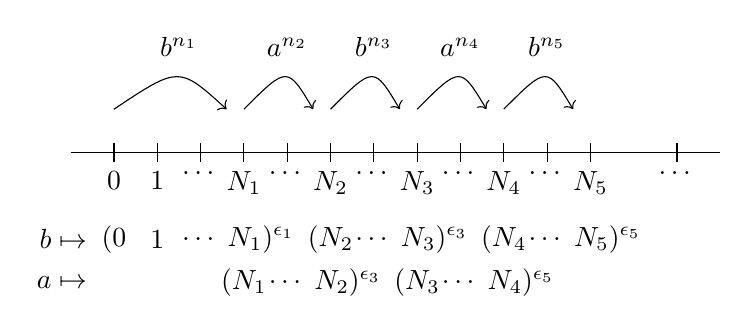
\begin{tikzpicture}[scale = 1.1]
\draw (-.5,0) -- (7,0) ;

\draw[shift={(0,0)},color=black] (0pt,3pt) -- (0pt,-3pt);
\draw[shift={(0,0)},color=black] (0pt,0pt) -- (0pt,-3pt) node[below] 
{$0$};
\draw[shift={(0.5,0)},color=black] (0pt,3pt) -- (0pt,-3pt);
\draw[shift={(0.5,0)},color=black] (0pt,0pt) -- (0pt,-3pt) node[below] 
{$1$};
\draw[shift={(1,0)},color=black] (0pt,3pt) -- (0pt,-3pt);
\draw[shift={(1,0)},color=black] (0pt,0pt) -- (0pt,-3pt) node[below] 
{$\dots$};
\draw[shift={(1.5,0)},color=black] (0pt,3pt) -- (0pt,-3pt);
\draw[shift={(1.5,0)},color=black] (0pt,0pt) -- (0pt,-3pt) node[below] 
{$N_1$};
\draw[shift={(2,0)},color=black] (0pt,3pt) -- (0pt,-3pt);
\draw[shift={(2,0)},color=black] (0pt,0pt) -- (0pt,-3pt) node[below] 
{$\dots$};
\draw[shift={(2.5,0)},color=black] (0pt,3pt) -- (0pt,-3pt);
\draw[shift={(2.5,0)},color=black] (0pt,0pt) -- (0pt,-3pt) node[below] 
{$N_2$};
\draw[shift={(3,0)},color=black] (0pt,3pt) -- (0pt,-3pt);
\draw[shift={(3,0)},color=black] (0pt,0pt) -- (0pt,-3pt) node[below] 
{$\dots$};
\draw[shift={(3.5,0)},color=black] (0pt,3pt) -- (0pt,-3pt);
\draw[shift={(3.5,0)},color=black] (0pt,0pt) -- (0pt,-3pt) node[below] 
{$N_3$};
\draw[shift={(4,0)},color=black] (0pt,3pt) -- (0pt,-3pt);
\draw[shift={(4,0)},color=black] (0pt,0pt) -- (0pt,-3pt) node[below] 
{$\dots$};
\draw[shift={(4.5,0)},color=black] (0pt,3pt) -- (0pt,-3pt);
\draw[shift={(4.5,0)},color=black] (0pt,0pt) -- (0pt,-3pt) node[below] 
{$N_4$};
\draw[shift={(5,0)},color=black] (0pt,3pt) -- (0pt,-3pt);
\draw[shift={(5,0)},color=black] (0pt,0pt) -- (0pt,-3pt) node[below] 
{$\dots$};
\draw[shift={(5.5,0)},color=black] (0pt,3pt) -- (0pt,-3pt);
\draw[shift={(5.5,0)},color=black] (0pt,0pt) -- (0pt,-3pt) node[below] 
{$N_5$};
\draw[shift={(6.5,0)},color=black] (0pt,3pt) -- (0pt,-3pt);
\draw[shift={(6.5,0)},color=black] (0pt,0pt) -- (0pt,-3pt) node[below] 
{$\dots$};

\draw[->] (0, .5) .. controls (.75,1) .. (1.3, .5);
\draw[->] (1.5, .5) .. controls (2,1) .. (2.3, .5);
\draw[->] (2.5, .5) .. controls (3,1) .. (3.3, .5);
\draw[->] (3.5, .5) .. controls (4,1) .. (4.3, .5);
\draw[->] (4.5, .5) .. controls (5,1) .. (5.3, .5);

\node[above] at (.75, 1) {$b^{n_1}$};
\node[above] at (2, 1) {$a^{n_2}$};
\node[above] at (3, 1) {$b^{n_3}$};
\node[above] at (4, 1) {$a^{n_4}$};
\node[above] at (5, 1) {$b^{n_5}$};

\node[left] at (-.2, -1) {$b \mapsto $};
\node[left] at (-.2, -1.5) {$a \mapsto $};

\node at (0, -1) {$(0$};
\node at (0.5, -1) {$1$};
\node at (1, -1) {$\dots$};
\node[right] at (1.2, -1) {$N_1)^{\epsilon_1}$};

\node at (2.5, -1) {$(N_2$};
\node at (3, -1) {$\dots$};
\node[right] at (3.2, -1) {$N_3)^{\epsilon_3}$};

\node at (4.5, -1) {$(N_4$};
\node at (5, -1) {$\dots$};
\node[right] at (5.2, -1) {$N_5)^{\epsilon_5}$};

\node at (1.5, -1.5) {$(N_1$};
\node at (2, -1.5) {$\dots$};
\node[right] at (2.2, -1.5) {$N_2)^{\epsilon_3}$};

\node at (3.5, -1.5) {$(N_3$};
\node at (4, -1.5) {$\dots$};
\node[right] at (4.2, -1.5) {$N_4)^{\epsilon_5}$};

\end{tikzpicture}


	\caption{Illustration of the action in the case of $F_2 = \left<a,b \right>$}
	\label{fig:}
\end{figure}

\end{example}

% example: finitely generated groups


\subsection{Properties of Residually Finite Groups}

It is a well-known result that residually finite groups are sofic. \todo{reference}% reference?

    \begin{theorem} \label{thm:res_fin_sofic}
        Every countable residually finite group is sofic.
    \end{theorem}
    \begin{proof}
        Let $G$ be a countable residually finite group. As $G$ is countable we can order the elements non-identity elements $g_1, g_2, g_3, \dots$ .
By the first property of residually finiteness, for every $i=1,2,3, \dots$ there exist a group $G_i$ and a homomorphism $f_i: G \to G_i$ such that $f_i(g_i) \ne 1_G$. Consider the direct products $H_n = \prod_{i = 1}^n G_i$ with the induced homomorphisms $h_i: G \to H_i: g \mapsto (f_1(g), f_2(g), \dots, f_i(g))$. Now we will look at the image of $G$ under these morphisms $\Gamma_i = h_i(G)$.


Notice that $\Gamma_i$ is always finite. We will implicitly identify $\sym(\Gamma_i)$ with $\sym(\card{\Gamma_i})$.
For every $i \in \N$, define $d_i = \card{\Gamma_i}$ and $\Phi_i: G \to \sym(\Gamma_i): g \mapsto (a \mapsto ga)$. We claim that this is a sofic approximation sequence for $G$.

For every $k \in \Gamma_i, g, h \in G$ we can see that $(\Phi_i(g) \circ \Phi_i(h))(k) = ghk = \Phi_i(gh)$. So
\[
\{k \in \Gamma_i \mid (\Phi_i(g) \circ \Phi_i(h))(k) = \Phi_i(gh)\} = \Gamma_i.
\]
Then we can see that for all $g,h \in G$:
$$\lim_{i\to \infty} \frac{1}{d_i} \left|\left\{k \in \Gamma_i| (\Phi_i(g) \circ \Phi_i(h))(k) = \Phi_i(gh)\right\}\right| = 1.$$

For every $g \in G, g\ne 1$ there is an $N \in \N$ such that for every $i > N$, $h_i(G) \ne 1_G$. So it is clear that 
$$\lim_{i \to \infty} \frac{1}{d_i} \card{\left\{k \in \Gamma_i \mid \Phi_i(g) = gk \ne k\right\}} = 1.$$
For $g = 1_G$ we find that 
$$\lim_{i \to \infty} \frac{1}{d_i} \card{\left\{k \in \Gamma_i \mid \Phi_i(g) = k \ne k\right\}} = 0,$$
which proves the second condition. 

    \end{proof}

    % \subsection{Examples of Sofic Groups}

    % \todo{Deze sectie moet herwerkt worden naar een overview van groepen die sofisch zijn, met referenties naar de voorbeelden/stellingen waar ze werden aangehaald}

    % \begin{description}
    %     \item[Finite groups] Every finite group, $G$ satisfies the Følner criterion, as the taking $(G)_n$ as sequence satisfies the properties in \cref{def:folner}.
    %     \item[Cyclic groups] All finite cyclic groups are taken care of by the previous example. We only need to check $\Z,+$. This group is residually finite as for every $n \in \Z, n \ne 0$ we can consider the natural morphism $\Z \to \Z /(|n|+1)\Z: x \mapsto x \mod |n|+1$. 
    %     \item[The finite direct product of Sofic groups] Let $G, H$ be sofic groups with sequence $d_i, e_i$ and maps $\sigma_i, \phi_i$ such that the properties of \cref{def:Sofic} hold. It can be (easily) verified that the sequence $(d_i + e_i)_i$ and maps $\psi_i: G \times H \to \sym(d_i + e_i): x (x \le d_i) \mapsto \sigma_i(x), x (x > d_i) \mapsto \phi_i(x -d_i) + d_i$ satisfy \cref{def:Sofic}.
    %     \item[Finitely generated free groups] They are residually finite.
    % \end{description}

 

    \section{Surjunctivity}\label{sec:surjunctivity}

    First we define a basic concept in group theory.

    \begin{definition} % van wikipedia gehaald
	    Let $G$ be a group and $X$ be a set. Then $\alpha: G \times X \to X: (g,x) \mapsto \alpha_g(x)$ is called an \textbf{right (group)action} of $G$ on $X$ if
        \begin{enumerate}[(i)]
		\item $\forall x \in X: \alpha_{1_G}(x) = x$
            \item $\forall g,h \in G, x\in X: \alpha_{hg}(x) = \alpha_g(\alpha_h(x))$.
        \end{enumerate}
    \end{definition}

    In this section we will encounter the set of all maps from $G$ to a finite set $A$. This set will be denoted by $A^G$. We will consider this set as a topological space, the topology on $A^G$ being the product topology, where $A$ carries the discrete topology. We will use ``sequence''-style notation and denote the elements of $A^G$ by $(x_g)_{g \in G}$ or $(x_g)_g$.

    \begin{definition}
	    Let $G$ be a countable group and $A$ a finite set. Then the \textbf{right shift} $\sigma$ of $G$ on $A^G$ is defined by
        \[
        \sigma: G \times A^G \to A^G: \left(g, (x_{h})_{h \in G} \right) \mapsto \sigma_g((x_{h})_{h \in G}) = \left( x_{hg} \right)_{h \in G}.
        \]
        %where $\sigma_g$ is defined by $\sigma_g\left( (x_{h})_{h \in G} \right) = \left( x_{hg} \right)_{h \in G}$.
        % Misschien is de ``rij-notatie'' hier niet aangewezen
    \end{definition}

    One can see that the right shift $\sigma$ is a right action of $G$ on $A^G$. We say that a map $\phi: A^G \to A^G$ \emph{commutes with the right shift} if $\sigma_g \circ \phi = \phi \circ \sigma_g$ for every $g \in G$.
    
    \begin{definition}
	    Let $G$ be a countable group. The group $G$ is called \textbf{surjunctive} if for any finite set $A$ and every injective and continuous $\phi: A^{G}\to A^{G}$ that commutes with the right shift $\sigma$ of $G$ on $A^G$ is also surjective.
	    \footnote{There is an alternative way to define this in terms of the \emph{left shift} $\tau$ defined by $\tau_g(h)= g^{-1}h$. This approach is completely equivalent and is followed by \cite{capraro_lupini_2015}.}
    \end{definition}\todo{reference} 

    % Szabo: reference

    \begin{conjecture}[Gottschalk] \label{conj:gottschalk}
        Every countable group is surjunctive.
    \end{conjecture}

    It can be proven that every sofic group is surjunctive. However, the proof is not easy. For that reason we will prove it first for the special case of residually finite groups. We will need the following definition
\begin{definition}
    Let $G$ be a countable group and $A$ a finite set. Let $H$ be a normal subgroup of finite index. Then the set of \textbf{$H$-periodic points} is the following subset of $A^G$.
        \[
        P_H = \{ (x_g)_{g \in G} \in A^G  \mid \forall h \in H: \sigma_h((x_g)_g) = (x_g)_g\}
        \]
\end{definition}

% Notice that this means that any $\omega \in P_H$ can be factored into the natural quotient map $i: G \to \frac{G}{H}$ and a function  $f: \frac{G}{H} \to A$ such that $\omega = f \circ i$.
% As we require $H$ to be normal and of finite index, we get that $\frac{G}{H}$ is a finite set. 
% So $f$ is a function from and to finite sets.
% There are only a finite number of such functions. 
% Hence $P_H$ is a finite set.

Since $H$ is of finite index, there exist elements $g_1, g_2, \dots, g_n$ such that $G = \bigcup_{i=1}^n g_i H$. It is then sufficient to specify $x_{g_1}, x_{g_2}, \dots, x_{g_n}$ to uniquely determine an element $(x_g)_{g \in G}$ of $P_H$. Indeed, any $g \in G$ can be written as $g = g_ih$ for some $i$, and then we have $x_g = x_{g_ih} = x_{g_i}$. Thus $P_H$ is finite since $A$ has only finitely many elements.

A key lemma we will further need in our proof of theorem \ref{thm:res_fin_surjunctive} is the following:

\begin{lemma} \label{lem:h-periodic_points}
    % The $H$-periodic points are dense in $A^G$, where $A$ is a finite set and $G$ is a residually finite countable group.
	    %\todo{Szabo: Be more precise. In light of your previous remark you obviously don't mean what you write. You claim denseness for the set of all points which are periodic w.r.t. some H, or, the union of the H-periodic points over ALL H.}
    
Let $G$ be a countable group and $A$ a finite set. Then the set of all periodic points (with respect to all normal subgroups of finite index)
    \[
    \bigcup_{\substack{ H \triangleleft G \\ [G : H] < \infty}} P_H
    \]
is dense in $A^G$.
\end{lemma}
\begin{proof}
% 	Let $f:G \to A \in A^G$. We will prove that there exists a sequence of periodic points that converges to $f$. As $G$ is countable we can list its elements $G = \{1, g_1, g_2, g_3,\dots\}$. 
	Let $F_n = \{1, g_1, g_2, \dots, g_n\}$ and fix $n$. 
	As $G$ is residually finite, for every $g \in F_n^{-1} \cdot F_n,\ g \ne 1$, we can find a map $\pi_g: G \to H_g$, where $H_g$ is a finite group and $\pi_g(g) \ne 1$.  Consider the map \[\pi = \prod_{ \substack{g\in  F_n^{-1} \cdot F_n\\ g\ne 0}} \pi_g
 .\]
	Observe that $\im \pi$ is finite, thus $\ker\pi$ is a normal subgroup of finite index of $G$. 
	For $g_i, g_j \in F_n, i \ne j$ it is clear that $\pi(g_i) \ne \pi(g_j)$ as $\pi(g_j^{-1} g_i) \ne 1$.
	This means that $\pi|_{F_n}: F_n \to \pi(F_n)$ is a bijection. 
	Define $\beta_n: \pi(F_n) \to A: h \mapsto \left(f \circ \left( \pi|_{F_n} \right)^{-1}\right)(h) $.
	Notice that for all $g_i \in F_n: (\beta \circ \pi)(g_i) = f(g_i)$.
	Take any extension  $\alpha_n: \im(\pi) \to A$ of  $\beta_n$.
        Notice that $\alpha_n \circ \pi \in A^G$. 
        Let $h \in \ker\pi$ and consider the right $h$ shift, $\sigma_h$. 
        Take any $g \in G$. 
        Then 
        \[\sigma_h(\alpha_n\circ\pi)(g) = (\alpha_n \circ \pi)(hg) = \alpha_n(\pi(h)\pi(g)) = \alpha_n(\pi(g)) = (\alpha_n\circ\pi)(g).\] Thus $\sigma_g(\alpha_n \circ \pi) = (\alpha_n\circ\pi)$.
        So $\alpha_n\circ\pi$ is a $\ker\pi$-periodic point. 

	For every $F_n =  \{1, g_1, g_2, \dots, g_n\}$ we can construct such a function $\alpha_n \circ \pi_n$ which is an $\ker \pi_n$ periodic point and that agrees with $f$ on $F_n$. 
	It is clear that $(\alpha_n \circ \pi_n)_{n\in\N}$ converges to $f$ pointwise as a function. 
	This is sufficient to say that $(\pi_n)_n$ converges to $f$ in the product topology.
Let $(x_g)_g \in A^G$ be arbitrary. Consider a basis open
\[
			U= \prod_{g \in G} \begin{cases}
				\{x_f\} & f \in F\\
				A & \text{ otherwise,}
			\end{cases}
			\] 
where $F$ is a finite subset of $G$. Now let $F^{-1}F\setminus\{e\} = \{g_1, \dots, g_n\}$. For $i=1, \dots, n$, we can find a finite group $H_i$ and a homomorphism $\alpha_i:G \to H_i$ such that $\alpha(g_i) \neq 1$. Now consider
\[
	\alpha: G \to \prod_{i=1}^n  H_i: g \mapsto (\alpha_1(g), \alpha_2(g), \dots, \alpha_n(g)).
\]

Since $\im \alpha$ is finite, $\ker \alpha$ is a normal subgroup of finite index. Moreover, for any $f_1 \neq f_2 \in F$, we have $\alpha(f_1^{-1}f_2) \neq 1$ and consequently $f_1 \ker \alpha \neq f_2 \ker \alpha$. Now we can write $G$ as a disjoint union
\[
 	G = \bigcup_{d \in D} d \ker \alpha,
 \] 
 where $D \supset F$ is a finite subset of $G$.
 Now we can define the $\ker \alpha$-periodic point $(y_g)_g$ uniquely by $y_d = x_d$ for every $d \in D$. Clearly, $(y_g)_g \in U$. Thus the set of periodic points with respect to all normal subgroups of finite index is dense in $G$.
\end{proof}

Now we can quite easily prove the following result. We follow the proof of Weiss \cite[Theorem 1.3]{weiss_2000} here.
\begin{theorem} \label{thm:res_fin_surjunctive}
    Every residually finite group is surjunctive.
\end{theorem}
\begin{proof}
    Let $G$ be a residually finite group and $A$ a finite set. Let $\phi: A^G \to A^G$ be a continuous map which commutes with the right shift $\sigma$. Assume further that $\phi$ is injective. We need to prove that $\phi$ is also surjective. Since $\phi$ commutes with the shift, it follows readily that it maps $H$-periodic points to $H$-periodic points, for any subgroup $H$ of finite index.
Because $P_H$ is finite (for $H$ of finite index), and $\phi$ is injective, the restriction of $\phi$ to $P_H$ is surjective, thus $P_H \subset \phi(A^G)$. Now since $A^G$ is compact, continuous maps from $A^G$ to itself map closed sets to closed sets. Therefore
\[
\phi(A^G) = \overline{\phi(A^G)} \supset
\overline{\bigcup_{\substack{\text{subgroup } H \\ [G : H] < \infty}}\phi( P_H)}
= \overline{\bigcup_{\substack{\text{subgroup } H \\ [G : H] < \infty}} P_H} = A^G,
\]
where we have used lemma \ref{lem:h-periodic_points}. Thus we conclude $\phi$ is surjective.

\end{proof}

\todo[color=green]{Apply this proof to Z!}
	
\section{Surjunctivity of Amenable and Sofic Groups}

\todo{Szabo:The phrasing here suggests that what you are about to do has something novel to it. Is that really the case? If so, point out explicitly what it is.}

In subsection \ref{ssec:amenable_surjunctive} we present a proof of the fact that amenable groups are surjunctive. In the literature, it is usual to do this using the concept of entropy (as in \cite[section 4]{kerr_li_2010} or \cite[subsection 2.13]{capraro_lupini_2015}), or using graph theory (as in \cite[section 3]{weiss_2000}). However, we came up with an alternative approach, independent of the literature, and will prove this well-known result directly from our definitions. We were unable to find a proof in the literature that follows the same approach, but it is important to point out that our proof and the aforementioned proofs have many conceptual similarities. 

Alas, we were unable to generalise these techniques to show that sofic groups are surjunctive. In subsection \ref{ssec:sofic_surjunctive}, we sketch how one can obtain the surjunctivity result for sofic groups using the concept of entropy.


\subsection{Amenable Groups are Surjunctive} \label{ssec:amenable_surjunctive}
In the following section $G$ will be a fixed countable amenable group, $A$ a fixed finite set and $\phi: A^{G} \to A^{G}$ a fixed continuous injective function that commutes with the right shift. 
We will also denote a fixed element of $A$ with $0$.

\begin{lemma}
	There exists a finite subset $\Gamma \subset G$ such that the value of $\phi((x_g)_{g \in G})(1_G)$ is only dependent on the values of $x_h$ where  $h \in \Gamma$, 
	i.e. if for some  $(x_g)_{g \in G}, (y_g)_{g \in G} \in A^{G}$ it holds that $x_h = y_h$ for all $h \in \Gamma$, then $\phi((x_g)_{g \in G})(1_G) = \phi((y_g)_g)(1_G)$.
\end{lemma}
\begin{proof}
	Choose any $a \in A$. As $\phi$ is continuous we know that \[
	U_a = \phi^{-1}\left( \prod_{g\in G} \begin{cases}
			\{a\} & g = 1_G\\
			A & g \ne 1_G
	\end{cases} \right)
\]
	is open. Hence we can choose some basis opens $U_{i, a}$ for some index $i \in I$ such that  \[
		U_a= \bigcup_{i \in I} U_{i,a}
	.\] 
	Notice that $\bigcup_{a \in A} U_a = A^{G}$ is a disjoint union. 
	Hence $\bigcup_{a \in A, i \in I} U_{i, a} = A^{G}$. 
	As $A^{G}$ is compact, we see that there must be a finite subset of indices $K$ such that \[
		A^{G} = \bigcup_{(i, a) \in K} U_{i, a}
	.\] 
	Every one of these basis opens is of the form \[
	U_{i,a} = \prod_{g \in G} \begin{cases}
		V_{i,a,g} & g \in \Gamma_{i,a}\\
		A & g \not\in \Gamma_{i,a}
	\end{cases}
	,\]
	for some open sets $V_{i,a,g} \subset A$ and finite subsets $\Gamma_{i,a} \subset G$. 

	We now claim that $\Gamma = \bigcup_{(i,a) \in K} \Gamma_{i,a}$ is set we are looking for. 
	Obviously $\Gamma$ is finite. 
	Further, suppose that $(x_g)_{g\in G} \in A^{G}$ and $(y_g)_{g \in G} \in A^{G}$ agree on $\Gamma$,
	meaning that for every $\gamma \in \Gamma$ it holds that  $x_\gamma = y_\gamma$.
	We know that for some  $(i, a) \in K$ the point $(x_g)_g \in U_{i,a}$. 
	In particular we see that $x_\gamma = y_\gamma$ for every $\gamma \in \Gamma_{i,a}$. 
	So $(y_g)_{g \in G} \in U_{i, a}$. 
	Hence  $(x_g)_{g \in G} , (y_g)_{g \in G}$ are elements of $U_a$. 
	So  $\phi((x_g)_{g \in G})(1_G) = a = \phi((y_g)_{g \in G})(1_G) $.
	We conclude that $\Gamma$ is indeed the set we're looking for.
\end{proof}
From this point on we will also fix $\Gamma$. 

\begin{corollary}
	For any $k \in G$ the value of $\phi((x_g)_{g \in G})(k)$ is only dependent on the values of $x_{kh}$ where $h \in \Gamma$.
\end{corollary}	
\begin{proof}
	As $\phi$ commutes with the right shift  $\sigma_k$ we know that $\sigma_k\phi = \phi\sigma_k$. Applying the previous lemma immediately gives the result.
\end{proof}

\begin{corollary}\label{cor:differ_in_image}
	If $(x_g)_{g \in G}, (y_g)_{g\in G} \in A^{G}$ only differ on a set $H \subset G$, ie $\forall g \not\in H:x_g = y_g$,
	then  $\phi((x_g)_{g \in G})$ and $\phi((y_g)_{g \in G})$ will only differ on $H\Gamma^{-1}$.
\end{corollary}
\begin{proof}
	Take $g \not\in H\Gamma^{-1}$. Then $\phi((x_h)_{h \in G})(g)$ and $\phi((x_h)_{h\in G})(g)$ will only depend on  $\{x_{g\gamma}\mid \gamma \in \Gamma\}$ and $\{y_{g\gamma}\mid \gamma \in \Gamma\} $. But  $g\Gamma \cap H = \emptyset$. Hence $x_{g\gamma} = y_{g\gamma}$ for all $\gamma \in \Gamma$. By the previous corollary we see that $\phi((x_h)_{h \in G})(g) = \phi((y_h)_{h \in G})(g)$.
\end{proof}

\begin{definition}
	We say that $(x_g)_{g \in G} \in A^{G}$ has support $H$ if $x_g = 0$ for all $g \not\in H$.
\end{definition}
Let $A_H$ be the set of all element of  $A^{G}$ with support $H$. We can implicitly identify $A_H$ with $A^{H}$.

\begin{lemma}\label{lem:injective_restriction}
	Let $H$ be any finite subset of $G$. Consider the function  \[
		\psi:A_H \to A ^{H\Gamma^{-1}}: (x_g)_{g \in G} \mapsto \left(h \mapsto \phi((x_g)_{g \in G})(h)\right)
	.\]  
	This function is an injection. 
\end{lemma}
\begin{proof}
	Suppose that $x= (x_g)_{g \in G}$ and $ y = (y_g)_{g \in G} \in A^{H}$ have the same image under $\psi$. As $x, y$ can only differ on $ H$, their images under $\phi$ cannot differ in $G\setminus H\Gamma^{-1}$ (see \cref{cor:differ_in_image}). Because they also have the same image under $\psi$, we know that $\phi(x)$ and $\phi(y)$ must also agree on $H\Gamma^{-1}$. Hence $\phi(x) = \phi(y)$. By the injectivity of $\phi$ we find that $x = y$.
\end{proof}

At this point we are almost ready to prove that $G$ is surjunctive, i.e.\ $\phi$ is surjective. 
In order to show this will show that for any finite subset $B\subset G$ and a map $f:B \to A$ we can find a $x \in A^{G}$ such that $\phi\left(x \right) |_B  = f$. Then we can finish the proof by showing that they image of $\phi$ is dense and using compactness.


\bigskip

For now, lets fix the set $B$ and the map $f:B \to A$. 
We will first introduce the notion of a copy of $B$. \footnote{This is not standard notation. It is just a term we made up to aid in this specific proof.}
 \begin{definition}
	A set  $A \subset  G$ is a copy of $B$ if and only if there exists an $s \in G$ such that $A = B\cdot s$.
\end{definition}


\begin{lemma}\label{lem:copies_of_B}
	Let $F$ be any finite subset of $G$. There exists a subset $F' \subset F$ such that for any two  $s,t \in F', s\ne t$ it holds that $B\cdot s$ and  $B\cdot t$ are disjoint and $\card{F'} \ge \frac{\card{F}}{\card{B}^2} $
\end{lemma}
In other words, the set  $BF$ contains at least $\frac{\card{F}}{\card{B^2}}$ disjoint copies of $B$.

\begin{proof}
	 We will prove this using strong induction. The case where $F = \emptyset$ is trivial. 
	\begin{description}
		\item{Case $1 \le \card F \le \card{B}^2$:} 
		Let  $f \in F$ be an arbitrary element of $F$. 
		The set $\{f\} $ has 1 element which is atleast $\frac{\card F}{\card B^2} \le 1$.
	\item{Case $\card F > \card{B}^2$ :}
		Take any  $f \in F$. Suppose that for some  $s \in G$,  $Bf$ and  $Bs$ are not disjoint. 
		Hence there exists $a,b \in B$ such that $af = bs$. 
		Thus $s = b^{-1}af$. So $s \in fB^{-1}B$. Notice that $\card{fB^{-1}B}\le \card{B}^2$.
		This means that for any $f' \in F \setminus fB^{-1}B$, $Bf$ and $Bf'$ will be disjoint. 
		Notice that $\card F > \card{F \setminus f B^{-1}B} \ge \card F - \card{B}^2 $.

		Applying the induction hypothesis shows that there exists a $F'\subset  \left( F\setminus fB^{-1}B \right) $ such that  for all  $s, t \in F'$, $Bs$ and $Bf$ are disjoint, 
		and that \[\card {F'}  \ge \frac{\card{F \setminus fB^{-1}B }}{\card{B}^2}.\]
		On top of that for every $f' \in F\setminus fB^{-1}B$, $Bf$ and  $Bf'$ will be disjoint. 
		So for every  $ s, t \in \{ f\} \cup F'\} $,  $Bs$ and $Bt$ will be disjoint.
		Further \[
			\card{\{f\} \cup F'}  = 1 + \card{F' } \ge 1 + \frac{\card{F \setminus fB^{-1}B}}{\card B^2} \ge \frac{\card{F}}{\card{B}^2}
		.\] 
		We conclude that $\{f\} \cup  F'$ is the set we are looking for. 
	\end{description}
\end{proof}


We are finally setup to proof that all amenable groups are surjunctive.
\begin{theorem}
	Let $G$ be a countable amenable group and  $A$ be finite set, where we will choose one element and denote it with $0$. Let  $\phi: A^{G} \to A^{G}$ be a injective, continuous map that commutes with the right shift. Then $\phi$ is surjective.
\end{theorem}

\begin{proof}
	Lets fix a finite subset $B \subset G$ and a map $f:B\to A$. 
	Suppose that there does not exists a  $x \in A^{G}$ such that $\phi(x)|_B = f$.
	Notice that this means that for any copy of $B$, take  $B\cdot s$, the image of $\phi$ does not contains a function  $\phi(x)$ such that when restrited to  $B\cdot s$ it is $f': B\cdot s \to A: x \mapsto f\left( x s^{-1} \right) $, as applying the right shift $\sigma_{s^{-1}}$ then gives $\phi(\sigma_{s^{-1}} x) |_{B} = f$.

	Let $F_n$ be a right Følner sequence of $G$. By \cref{cor:product_folner_sequence} we know that $BF_n$ is a right Følner sequence as well. 

	Fix  $n$ for a moment. By \cref{lem:injective_restriction} the function \[
		\psi: A^{BF_n} \to A^{BF_n\Gamma^{-1}}: x \mapsto (g \mapsto \phi(x)(g))
	.\] 
	is injective.
	\Cref{lem:copies_of_B} states that we can choose  $ \left\lceil \frac{\card{F_n\Gamma}}{\card{B}^2} \right\rceil $ disjoint copies of $B$ in $BF_n\Gamma$. 
	We know that for every such copy of $B$ the number of possible values at the coordinates of this copy is atmost  $\card{A}^{\card{B}} -1$ by our assumption at the start of this proof.
	Hence there exists a set $\mathcal{A} \subset A^{BF_n\Gamma^{-1}}$ of cardinality \[
		\card{\mathcal{A}} = \card{A}^{\card{BF_n\Gamma^{-1}}- \card{B}\left\lceil \frac{\card{F_n\Gamma^{-1}}}{\card{B}^2} \right\rceil } \cdot (\card{A}^{B} -1)^{\left\lceil \frac{\card{F_n\Gamma^{-1}}}{\card{B}^2} \right\rceil }
\]
such that $\im\psi \subset \mathcal{A}$. 
As $\psi$ is injective it follows that $\card{A^{BF_n}} \le \card{\mathcal{A}}$. Hence
\[
	\card{A}^{\card{BF_n}} \le 
	\card{A}^{\card{BF_n\Gamma^{-1}}- \card{B}\left\lceil \frac{\card{F_n\Gamma^{-1}}}{\card{B}^2} \right\rceil } \cdot (\card{A}^{B} -1)^{\left\lceil \frac{\card{F_n\Gamma^{-1}}}{\card{B}^2} \right\rceil }
.\]
By taking the logarithm of both sides we obtain
\[
	\card{BF_n}\ln(\card{A}) \le \card{BF_n\Gamma^{-1}} \ln(\card{A}) - \left\lceil \frac{\card{F_n\Gamma^{-1}}}{\card{B}^2} \right\rceil \left( \ln(\card{A}^{\card{B}}) - \ln(\card{A}^{\card{B}} -1) \right)   
.\]
By dividing both sides by $\card{BF_n}$ we see 
\[
	\ln(\card{A}) \le \frac{\card{BF_n\Gamma^{-1}}}{\card{BF_n}} \ln(\card{A}) - \frac{1}{\card{BF_n\Gamma^{-1}}}\left\lceil \frac{\card{F_n\Gamma^{-1}}}{\card{B}^2} \right\rceil \left( \ln(\card{A}^{\card{B}}) - \ln(\card{A}^{\card{B}} -1) \right)   
.\]
\Cref{lem:folner_finite_subset} shows that $\lim_{n \to \infty} \frac{\card{BF_n\Gamma^{-1}}}{\card{BF_n}} = 1$. 
So we know as well that $\lim_{n \to \infty} \frac{1}{\card{BF_n\Gamma^{-1}}} \left\lceil \frac{\card{F_n\Gamma^{-1}}}{\card{B}^2} \right\rceil \ge \frac{1}{\card{B}^3} $. 
Therefore \[
	\ln(\card{A}) \le \ln(\card{A}) - \frac{1}{\card{B}^3} \left(\ln(\card{A}^{\card{B}}) - \ln(\card{A}^{B} - 1) \right)
,\]
which yields a contradiction. 
So our initial assumption is false. 

\bigskip

This means that there exists a $x \in A^{G}$ such that $\phi(x)|_B = f$. As this is true for every  $B$ and $f:B\to A$ we see that the image of  $\phi$ must be dense in $A^{G}$. As a map on compact spaces maps closed sets to closed sets we see that the image of $\phi$ must be $A^{G}$. 
We conclude that $\phi$ is surjective!


\end{proof}


\subsection{Sofic Groups, Entropy and Surjunctive Groups}\label{ssec:sofic_surjunctive}

To prove that sofic groups are always surjunctive we define sofic entropy. The definition we present is a particular case of the more general definition formulated in paragraph 2.13.6 in \cite{capraro_lupini_2015} and is equivalent to the one given in definition 4.2 of \cite{kerr_li_2010}. 

\begin{definition}

A subshift $X \subset A^G$ with $A$ a finite set and $G := \{g_0 = 1_G, g_1, g_2, ...\}$ any countable group is a closed subset which is invariant under the shift.\\
\\
Suppose now that $G$ is sofic and $\Sigma := (\Phi_i: G \to \sym(d_i))_{i \in \N}$ is a sofic approximation sequence. Take a subshift $X$ and a finite subset $F \subset G$. For any $\delta > 0$ and $n \in \N$ we define the set 
		\[
		H_n (\delta) := \{(a_i)_{0 \leq i \leq n-1} \in A^n | 
						\exists (x_i)_{0 \leq i \leq n-1} \in X_n : 
						\forall g \in F: d((a_{\Phi^{-1}_n(g)(i)})_i,(x_{ g_i g})_i) < \delta \}
		\]
		% \[
		% H_n (\delta) := \{(a_0, a_1, \dots, a_{n-1}) \in A^n \mid
		% 				\exists (x_0, x_1, \dots, x_{n-1}) \in X_n : 
		% 				\forall g \in F: d_{S_n}((a_{\Phi^{-1}_n(g)(i)})_i,(x_{g g_i})_i) < \delta \}
		% \]
		where by $X_n \subset A^n$ we mean the sequences in $X$ restricted to $\{1_G, g_1, g_2, ..., g_{n-1}\}$ (and we identify $x_{g_i}$ with $x_i$ for all $0 \leq i \leq n-1$). By the distance $d((x_i)_i, (y_i)_i)$ between two sequences $(x_i)_{0 \leq i \leq n-1}$ and $(y_i)_{0 \leq i \leq n-1}$ is meant the number of different components relative to their length:
		\[
		d((x_i)_i, (y_i)_i) = \frac{1}{n} |\{i \in \{0, ..., n-1\}|x_i \neq y_i\}|
		\]
				

		Now we define entropy as 
		\[
		h_\Sigma(X) := \inf_{\delta>0} \limsup_{n \to \infty} \frac{1}{n} \log |H_n(\delta)|
		\]
\end{definition}

It should be noted that in the definition of $H_n(\delta)$ provided above the right shift $\sigma_g$ is used on the sequence $(x_i)_i$, whereas the definition in \cite[paragraph 2.13.6]{capraro_lupini_2015}.\\

We shall use the following intermediate result, for which a sketch of the proof is provided. For the complete proof, we refer to either \cite[paragraph 2.13.7]{capraro_lupini_2015} or \cite[theorem 4.12]{kerr_li_2010}.

\begin{lemma}
For $X \subset A^G$ a subshift we have that 
		\[
		h_\Sigma(X) = \log |A| \Leftrightarrow X = A^G
		\]
\end{lemma}
\begin{proof}
For the implication $X = A^G \Rightarrow h_\Sigma(X) = \log |A|$: assume that $X = A^G$. Now it is quite clear that for any $n \in \N$ and $\delta > 0$: $|H_n(\delta)| = |A|^n$. Indeed, for any $(a_i)_i \in A^n$ we can find a sequence $(x_i)_i \in X^n$ such that $\forall g \in F: d_{S_n}((a_{\Phi^{-1}_n(g)(i)})_i,(x_{g_i g})_i) < \delta$. Namely  $(a_i)_i$ itself. Therefore $h_\Sigma(X) = \log |A|$.\\
\\
For the implication $h_\Sigma(X) = \log |A| \Rightarrow X = A^G$: assume that $X \varsubsetneq A^G$. It is possible that a certain element of $A$ is never a component in one of the elements of $X$. However, then it is immediately clear that $h_\Sigma(X) \leq \log (|A|-1) $ and thus $h_\Sigma(X) < \log |A|$. Assume, therefore, that every element of $A$ is a component in at least one of the elements of $X$. Now there must exist some finite $F \subset G$ such that $Y_F \varsubsetneq A^G$. It can then be shown that, using this $F$, we have that
		\[
		h_\Sigma(X) \leq \log |A| - \frac{1}{|F|^2} \log \left(\frac{|A|^{|F|}}{|A|^{|F|} - 1}\right) < \log |A|
		\]
which proves the implication by contrapositive. 
\end{proof}

Now we can prove the surjunctivity of sofic groups.

\begin{theorem}
Any sofic group G is surjunctive.
\end{theorem}
\begin{proof}
Suppose that we have a map $\phi: A^G \to A^G$ which is continuous, injective and which commutes with the shifts $\sigma_g$. Now consider $X := \phi(A^G) \subset A^G$. We claim that this is a subshift. Indeed, because $\phi$ is continuous and $A^G$ is compact, $X$ is closed. Furthermore, $X$ is invariant under any shift $\sigma_g$: 
		\begin{align*}
		\sigma_g(X)
		&= (\sigma_g \circ \phi) (A^G) \\
		&= (\phi \circ \sigma_g)(A^G) \\
		&= \phi(A^G).
		\end{align*}
		
The inverse $\phi^{-1}: X \to A^G$ is well defined, continuous (since $A^G$ and therefore also $X$ is Hausdorff) and commutes with the shifts. Therefore,  $\phi^{-1}$ is determined by a finite restriction $\phi^{-1}_0: X_{\Gamma} \to A^{\Gamma}$ with $\Gamma$ a finite subset of $G$. Indeed, since $\phi^{-1}$ is continuous, the value of any component, say $(\phi^{-1}((x_g)_{g \in G}))_e \in A$ is determined by the values $(x_g)_{g \in \Gamma}$ of a finite subset $\Gamma \subset G$, meaning 
		\[
		(\phi^{-1}((x_g)_{g \in G}))_e = (\phi^{-1}_0((x_g)_{g \in \Gamma}))_e
		\]

Now, take a sequence $(x_g)_{g \in G} \in X$ and its restriction $(x_g)_{g \in \Gamma} \in X_{\Gamma}$. Now for any $h \in G$ it is the case that 
		\[
		(\phi^{-1}((x_g)_{g \in G}))_h = (\sigma_h \circ \phi^{-1}((x_g)_{g \in G}))_e  = (\phi^{-1} \circ \sigma_h((x_g)_{g \in G}))_e
		\]

This knowledge allows us to write
		\begin{align*}
		(\phi^{-1}((x_g)_{g \in G}))_h
		&= (\sigma_h \circ \phi^{-1}((x_g)_{g \in G}))_e \\
		&= (\phi^{-1}((x_{gh})_{g \in G}))_e \\
		&= (\phi^{-1}_0((x_{gh})_{g \in \Gamma}))_e \\
		&= (\phi^{-1}_0((x_g)_{g \in \Gamma h}))_e
		\end{align*}
Now fix any $\delta > 0$. Consider $H_n(\delta)$ for any $n \in \N$. Look at any sequence $(a_i)_i \in A^n$. As $\Gamma$ is only finite, there exists a $N \in \N$ such that $g_N \in \Gamma$ and for any $g_i \in \Gamma: i \leq N$. Now take $n \geq N$. There exists a sequence $(x_i)_i \in X_n$ for which it is true that $x_i = a_i$ for any $i(0 \leq i \leq n)$ such that $g_i \in \Gamma$. It is quite clear now that $d((a_{\Phi^{-1}_n(g)(i)})_i,(x_{g_i g})_i)) < \delta$ for every $g \in \Gamma$ as long as we choose $n \in \N$ large enough. This is equivalent to saying that for $n \in \N$ large enough $(a_i)_i \in H_n(\delta)$ for every $(a_i)_i \in A^n$ . Therefore, $\limsup_{n \to \infty} |H_n(\delta)| = |A|^{n}$ for any $\delta >0$ and $h_\Sigma(X) = \log |A|$, which, by the previous lemma, means that $X = A^G$. Thus, $\phi$ is surjective.


\end{proof}

	\section{Kaplansky's Direct Finiteness Condition for Finite Fields}
	Let us recall the statement of Kaplansky's direct finiteness condition.
	\begin{definition}
		Let $\mathbb K$ be a field and $G$ be a group. The group ring $\mathbb K[G]$ is called \textbf{directly finite} if every  $a \in K[G]$, that is left invertible, is right invertible as well. 
		
	\end{definition}
	Kaplansky conjectured that all group rings are directly finite and Weiss showed that this is true for all sofic groups \cite[section 3, section 4]{weiss_2000}. 
	In the case where $\mathbb K$ is a finite field, Weiss did this by first proving the the surjunctivity of sofic groups.
	He finished the argument by proving that the group rings of finite fields and surjunctive groups are directly finite.  

	In this section we will give the details of a proof of that last step. 
	i.e we will prove the following theorem. 
	\begin{theorem}\label{thm:gottschalk_kaplansky}
		Let $\F$ be a finite field and $G$ be a surjunctive group. Then $\F[G]$ is directly finite. 
	\end{theorem}
	%It looks like we will need to use the surjuctivity on $\F^{G}$. Hence we need some statement that relates $\F^{G}$ to $\F[G]$.
	To exploit the surjunctivity property of $G$, we will need to relate $\mathbb F^G$ to the group ring $\mathbb F[G]$. There is in fact a very nice connection that can be made for any field $\mathbb K$.
	For finite groups, one can very naturally identify $\mathbb K^G$ with the group ring $\mathbb K[G]$. Indeed, with every element $(x_g)_{g \in G}$ in $\mathbb K^G$, there corresponds an element $\sum_{g \in G} x_g g$ in $\mathbb K[G]$, where $G$ being finite guarantees that this is a finite linear combination. For infinite groups, we cannot identify these two sets, but we can consider $\mathbb{K}[G]$ as a subset of $\mathbb K^G$. In this case, $\mathbb K^G$ is not a ring but we can make it into a module over $\mathbb K[G]$. We can do this in very natural way, extending the multiplication as defined in \cref{def:group_ring}. Here, one can think of the elements of $\mathbb K^G$ as (possibly infinite) formal sums $\sum_{g \in G} x_g g$ in $\mathbb K[G]$.

	\begin{lemma}
		For a group $G$ and field $\mathbb K$ we can consider $\mathbb{K}^{G}$ as a left $\mathbb{K}[G]$-module, with pointwise addition and multiplication defined as
		\begin{align*}
			\cdot : (\mathbb{K}[G] , \mathbb{K}^{G}) &\longrightarrow \mathbb{K}^{G} \\
		\left( \sum_{g \in G} a_g g,  (x_g)_{g \in G}\right)  &\longmapsto \left( \sum_{h \in G} a_h x_{h^{-1}g} \right)_{g \in G}
	.\end{align*} 
	\end{lemma}
	\begin{proof}
		The proof is given in appendix \hyperlink{sec:module}{C}.
	\end{proof}
    %     \begin{remark}
    %     The way $\F^{G}$ is defined as a $\F[G]$-module is not completely abitrary. It should be easy to see that  $\F^{G}$ can be represented as formal sums $\sum_{g \in G} x_g g$, just like $\F[G]$, but where we now allow infinite sums. 
    %     The definition of the multiplication between $\F[G]$ and  $\F^{G}$ agrees with the obvious multiplication with $\F^{G}$ represented as above. 
    % \end{remark}
    
	We are now ready to give a proof of \cref{thm:gottschalk_kaplansky}.
	\begin{proof}
		Let $\F$ be a finite field and $G$ be a surjunctive group. 
		Let $a = \sum_{g \in G} a_g g \in \F[G]$ be a left invertible element with left inverse $b$, i.e.  $b a = 1$. 
		Consider the map $\phi: \F^{G} \to \F^{G}: x \mapsto a\cdot x$. Notice that this map 
		\begin{itemize}
			\item is injective. Suppose that $\phi(x) = \phi(y)$. Then $a\cdot x = a\cdot y$. So $ba\cdot x  = x$ and $ba \cdot y = 1\cdot y = y$. Hence $x = y$.
			\item commutes with the bernoulli shift  $\sigma_k$. 
				 \[
					 \sigma_k \phi(x) 
					 = \sigma_k\left( \sum_{h \in G} a_h x_{h^{-1}g} \right)_{g \in G} 
					 = \left( \sum_{h \in G} a_h x_{h^{-1}gk} \right)_{g \in G} 
					 = \left( \sum_{h \in G}a_h h \right) \cdot (x_{gk})_{g \in G} = \phi(\sigma_k(x)) 
				\]
			\item is continuous. 
			One can easily check that the set $\left\{ U_{h, t} \right\}$, where \[
			U_{h,t}:= \prod_{g \in G} \begin{cases}
				\F & h \ne g\\
				\{t\}& h = g
			\end{cases}
			.\] 
			is a subbasis of $\F^{G}$. 
			Hence, to prove that $\phi$ is continuous it is sufficient to check that $\phi^{-1}(U_{h, t})$ is open for every $h \in G, t\in \F$.
			Notice that an  $(x_g)_{g \in G} \in \F^{G}$ is in $\phi^{-1}(U_{h,t})$ if and only if $\sum_{k \in G} a_k x_{k^{-1}h} = t$. 
			Remember that $a_k$ is nonzero only for a finite number subset $X$,  $k\in X \subset G$. 	
			So $\phi^{-1}(U_{h, t})$ is closed under addition with an element of  \[
			\prod_{g \in G} \begin{cases}
				\F & hg^{-1}  \not\in X\\
				\{0\} & hg^{-1} \in X 
			\end{cases}
			.\] 
			Let  $(x_g) \in \phi^{-1}(U_{g,t})$. We see that  \[
				(x_g) \in \prod_{g \in G} \begin{cases}
					\F & hg^{-1} \not\in X\\
					\{x_g\} & hg^{-1} \in X
				\end{cases}
				\subset \phi^{-1}(U_{h, t})
			.\] 
			So $\phi^{-1}(U_{h,t})$ is open. Hence $\phi$ is continuous.			
		\end{itemize}
		By the surjunctivity of $G$ we find that $\phi$ is surjective as well. In particular this means that there exists a $y = (y_g)_{g \in G}$ such that $\phi(y) = (\delta_{g, 1})_{g \in G}$, where $\delta$ is the kronecker delta.
		By multiplying with $b$ on the left we find that \[
			 y = ba\cdot y = b\cdot (\delta_{g, 1})_{g \in G} = \left( \sum_{h \in G} b_{h} \delta_{h^{-1}g, 1} \right)_{g \in G} = \left( \sum_{h \in G} b_{h} \delta_{h, g} \right)_{g \in G}
		 = \left( b_{g} \right) _{g \in G}.\] 
		This means that \[
		a\cdot y = \left( \sum_{h \in G} a_h b_{h^{-1}g} \right)_{g \in G} = \left( \delta_{g, 1} \right) _{g \in G} 
	.\] 
	In other words
	\[
	\sum_{h \in G} a_h b_{h^{-1}g} = \delta_{g, 1}
	.\]
	But this means exactly that $ab = 1$. So  $a$ is right invertible as well. 
	\end{proof}	
	
	\section{Conclusion}

We shall now briefly discuss the contents and results of this report and how they contribute to our attempt to thoroughly examine Kaplansky’s direct finiteness conjecture and understand how it relates to the notion sofic groups.\\
\\
Firstly, we extensively explored the definition and properties of sofic  groups as well as closely related concepts. In particular, we investigated the amenability and residual finiteness of groups and their meaning in the context of this subject. In both cases, we ended our analysis with a proof of their implying soficity. \\
\\
Secondly, we drew the connection between sofic groups and Kaplansky’s conjecture via the notion of surjunctivity. Specifically, we have provided proof of both the implication $amenable \Rightarrow surjunctive$ as well as $sofic \Rightarrow surjunctive$ for any countable group using independent, respective approaches. More importantly, however, the core of the report closes with proof that surjunctive groups adhere to Kaplansky’s conjecture in the case of finite fields. \\
\\
Finally, we can now conclude this report with the issue of open problems which remain in this area of mathematical research. In discussing this subject, we have quite naturally come across Gottschalk’s conjecture, as it tightly links the question of general surjunctivity with Kaplansky’s conjecture. Namely, if every countable group could be shown to be surjunctive, this would immediately resolve Kaplansky’s conjecture for finite fields. Even more striking, however, is the idea that every group might be sofic as well, as there exist no known counterexamples – though Weiss does not seem particularly enthusiastic about this possibility \cite[introduction]{weiss_2000} -  . Soficity for all countable groups would settle the question of direct finiteness of their grouprings over any field, without further ado, rendering everything discussed in this report mostly superfluous.

	\newpage
	\appendix
	\appendixpage
	\addappheadtotoc
	%\addappheadtotoc
	
	\tocless\section{\hypertarget{sec:proof_groupring}{Group Rings are Rings}}	
	\addcontentsline{toc}{subsection}{\numberline{A} Group Rings are Rings}
	
	\begin{proof}
		We need to prove associativity of $+$, commutativity of $+$, existence of zero element, existence of additive inverses, associativity for $\cdot$, left distributivity, right distributivity and existence of a unit element.
		% further proof needed
		\begin{description}
		\item[associativity of $+$]
		\begin{align*}
		\left(\sum_{g \in G} \lambda_g g + \sum_{g \in G} \mu_g g\right)+ \sum_{g \in G} \nu_g g
		&= \sum_{g \in G} \left((\lambda_g g + \mu_g g)+\nu_g g\right) \\
		&= \sum_{g \in G} \left(\lambda_g g + (\mu_g g+\nu_g g)\right) \\
		&= \sum_{g \in G} \lambda_g g + \left(\sum_{g \in G} \mu_g g + \sum_{g \in G} \nu_g g \right)
		\end{align*}
	
		\item[commutativity of $+$]
		\begin{align*}
		\sum_{g \in G} \lambda_g g + \sum_{g \in G} \mu_g g
		&= \sum_{g \in G} (\lambda_g g + \mu_g g) \\
		&= \sum_{g \in G} (\mu_g g + \lambda_g g) \\
		&= \sum_{g \in G} \mu_g g + \sum_{g \in G} \lambda_g g 
		\end{align*}
	
		\item[existence of $0$]
		\begin{align*}
		\sum_{g \in G} \lambda_g g + \sum_{g \in G} 0 g
		&= \sum_{g \in G} (\lambda_g + 0)g \\
		&= \sum_{g \in G} \lambda_g g
		\end{align*}
	
		\item[existence of additive inverse]
		\begin{align*}
		\sum_{g \in G} \lambda_g g + \sum_{g \in G} (-\lambda_g g)
		&= \sum_{g \in G} (\lambda_g - \lambda_g) g \\
		&= 0
		\end{align*}
	
		\item[associativity of $\cdot$]
		\begin{align*}
		\left[\left(\sum_{g \in G} \lambda_g g \right) \cdot \left(\sum_{g \in G} \mu_g g \right)\right ] \cdot \sum_{g \in G} \nu_g g
		&= \left(\sum_{g \in G} \left( \sum_{h \in G} \lambda_{h} \mu_{h^{-1}g} \right) g \right) \cdot \sum_{g \in G} \nu_g g\\
		&= \sum_{g \in G} \sum_{x \in G} \left( \sum_{h \in G} \lambda_{h} \mu_{h^{-1}x} \right) \nu_{x^{-1}g} \,g \\
		&= \sum_{g \in G} \sum_{y \in G} \sum_{h \in G} \lambda_{h} \mu_{y} \nu_{y^{-1} h^{-1}g} \, g \\
		&= \sum_{g \in G} \sum_{h \in G} \lambda_h \left(\sum_{y \in G}\mu_{y} \nu_{y^{-1} (h^{-1}g)}\right)g \\
		&= \left(\sum_{g \in G} \lambda_g g \right) \cdot \left[ \left(\sum_{g \in G} \mu_g g \right) \cdot \sum_{g \in G} \nu_g g \right]
		\end{align*}
	
		\item[left distributivity]
		\begin{align*}
		\sum_{g \in G} \lambda_g g \cdot \left(\sum_{g \in G} \mu_g g + \sum_{g \in G} \nu_g g \right) 
		&= \sum_{g \in G} \lambda_g g \cdot \sum_{g \in G} (\mu_g + \nu_g) g \\
		&= \sum_{g \in G} \sum_{h \in G} \lambda_h (\mu_{h^{-1}g} + \nu_{h^{-1}g}) g \\
		&= \sum_{g \in G} \left(\sum_{h \in G} \lambda_h \mu_{h^{-1}g} + \lambda_h \nu_{h^{-1}g}\right) g \\
		&= \sum_{g \in G} \lambda_g g \cdot \sum_{g \in G} \mu_g g
			+ \sum_{g \in G} \lambda_g g \cdot \sum_{g \in G} \nu_g g
		\end{align*}
	
		\item[right distributivity]
		\begin{align*}
		\left(\sum_{g \in G} \lambda_g + \sum_{g \in G} \mu_g g\right) \cdot \sum_{g \in G} \nu_g g
		&= \left(\sum_{g \in G} (\lambda_g g + \mu_g) g\right) \cdot \sum_{g \in G} \nu_g g\\
		&= \sum_{g \in G} \sum_{h \in G} (\lambda_h + \mu_h) \nu_{h^{-1}g} g \\
		&= \sum_{g \in G} \sum_{h \in G} \lambda_h \nu_{h^{-1}g} g + \mu_h \nu_{h^{-1}g} g \\
		&= \sum_{g \in G} \lambda_g g \cdot \sum_{g \in G} \nu_g g + \sum_{g \in G} \mu_g g \cdot \sum_{g \in G} \nu_g 
		\end{align*}
	
		\item[existence of 1]
		\begin{align*}
		\sum_{g \in G} \delta_{g,1_G} g \cdot \sum_{g \in G} \lambda_g g
		&= \sum_{g \in G} \left(\sum_{h \in H} \delta_{h,1_G} \lambda_{h^{-1}g} \right) \\
		&= \sum_{g \in G} \lambda_{1_G^{-1}g} g = \sum_{g \in G} \lambda_g g.
		\end{align*}
		
		\end{description}
        \end{proof}

	\tocless\section{\hypertarget{sec:intro_free_group}{A Brief Introduction to Free Groups}} 
	\addcontentsline{toc}{subsection}{\numberline{B} A Brief Introduction to Free Groups} 

This section is a brief introduction to the free groups, as many of our readers may not be familiar with this family of groups. 
This is in no way meant to be a rigorous construction of the group and its properties, rather it is an informal overview of its construction and its most important property.
The details can be found in many algebra text books such as \cite[section 7.9]{artin_algebra_1991} or \cite[section 5.5]{rotman_advanced_2015}.

The construction of a free group starts with the notion of an \emph{alphabet}, which is a set of \emph{letters}/symbols. We usually denote the alphabet with $S$. In the case where the alphabet only contains two letters we usually denote these with  $a,b$. In other cases we usually index the letters $x_i$ for some index $i \in I$, such that  $S = \{x_i  \mid i \in I\} $.

Using the letters of the alphabet  $S = \{x_i \mid i \in I\} $ we can make \emph{words}. Words are finite sequences of letters and inverses of letters. At this point inverses of letters are just more symbols. We denote $W(S)$ for the words made with letters in $S$. For example if $S = \{a,b\} $ the following are words $a$, $b$, $a^{-1}$, $ab^{-1}$, $aa^{-1}b$, $aabba^{-1}$, $1$. Notice that there is also the empty word containing no letters (denoted by $1$). 
We define the \emph{reduction of a word}, $\red w$,  as the operation that repeatedly scraps any pairs of letters adjacent to its inverse, $x_ix_i^{-1}$ and $x_i^{-1}x_i$, until there are no more such pairs. 
For example $\red({a^{-1}ab}) = b$, $\red(a a^{-1}) =1$ $\red(aba^{-1}b^{-1}) = aba^{-1}b^{-1}$, $\red(a^{-1}bb^{-1}a^{-1}) = 1$, $\red(x_1x_2x_3) = x_1x_2x_3$.

We can define a \emph{multiplication} on words by concatenating the sequences and reducing the result. For example $(ab)\cdot (ba) = abba$, $(ab)\cdot(b^{-1}a) = \red(abb^{-1}a) = aa$.
Using this multiplication it turns out that we can define the \emph{free group generated by $S$} as  \[
	F_S = \{\text{reduced words in $W(S)$}\}, \cdot  
.\]
We also write $F_S = \left<S \right>$, or in the case $S = \{x_1, x_2, \ldots, x_n\} $, we write $F_S = \left<x_1, x_2, \ldots, x_n \right>$. If  $S$ is finite with  $n = \card{S}$, we also write  $F_n$ as for two alphabets of the same cardinality  $S, S'$ the groups $F_S$ and $F_{S'}$ are isomorphic.


In some sense, the free group, $F_S$ is the largest group that can be generated by the elements of $S$. This is formalized in the following \emph{universal property of the free group}, that characterizes the free group. 
\begin{property}[{\cite[ch. 5, p. 298]{rotman_advanced_2015}}]
	If  $S$ is a subset of a group  $F$, then $F$ is the free group generated by $S$ if and only if for every group $G$ and function $f:S \to G$ there exists a unique morphism $\phi:F \to G$ such that $\phi(s) = f(s)$ for all $s \in S$.
	I.e. such that $\phi$ makes the following diagram commute:
	\[	
	\begin{tikzcd}
		F \arrow[rd, "\phi"]  \\
		S \arrow[u, hook] \arrow[r, "f"] & G
	\end{tikzcd}
\]

\end{property}


\tocless\section{\hypertarget{sec:module}{$\mathbb K^G$ is a $\mathbb K[G]$-module}}
\addcontentsline{toc}{subsection}{\numberline{C} $\mathbb{K}^{G}$ is a $\mathbb{K}[G]$-module}
	We check the module axioms one by one.
        In the following calculations $r = \sum_{g \in G}^{} r_g g,\ s = \sum_{g \in G}^{} s_g g$ are arbitrary elements of $\mathbb{K}[G]$ and $x = (x_g)_{g \in G}, y = (y_g)_{g \in G}$ are arbitrary elements of $\mathbb{K}^{G}$.
        \begin{description}
            \item[left distributivity] 
                \begin{align*}
                    r\cdot (x+y) &= \left( \sum_{h \in G} r_h (x_{h^{-1} g} + y_{h^{-1} g}) \right)_{g \in G} \\
                             &= \left( \sum_{h \in G} r_h x_{h^{-1} g} \right)_{g \in G}  + \left( \sum_{h \in G} r_h y_{h^{-1}g} \right)_{g \in G}  \\
                             &= r\cdot x + r\cdot y 
                .\end{align*}
            \item[right distributivity]
                \begin{align*}
                    (r + s)\cdot x &= \left( \sum_{h \in G} (r_h + s_h) x_{h^{-1} g} \right)_{g \in G}  \\
                               &= \left( \sum_{h \in G} r_h x_{h^{-1}g} \right)_{g \in G} + \left( \sum_{h \in G} s_{h} x_{h^{-1}g}  \right)_{g \in G} \\ 
                               &= r\cdot x + s \cdot y 
                .\end{align*}
        
            \item[associativity]
                 \begin{align*}
                     (rs)\cdot x %&= \left( \sum_{g_1 \in G} \sum_{g_2 \in G} r_{g_1} s_{g_2} g_1 g_2 \right) \cdot (x_{g})_{g \in G} \\
                             &= \left( \sum_{h \in G} \sum_{k \in G} r_{k}s_{k^{-1}h} h\right) \cdot  \left( x_{g} \right)_{g \in G} \\
                             &= \left( \sum_{h \in G} \sum_{k \in G} r_k s_{k^{-1}h} x_{h^{-1}g} \right)_{g \in G}  \\
                             &= \left( \sum_{h \in G} \sum_{k \in G} r_k s_{k^{-1}h} x_{(k^{-1} h)^{-1}(k^{-1}g)} \right)_{g \in G}  \\
                             &= \left(\sum_{h \in G} r_h h\right) \cdot  \left( \sum_{k \in G} s_{k} x_{k^{-1}g} \right)_{g \in G} \\
                             &= r(s\cdot x) 
                .\end{align*}
            \item[unity]
                \begin{align*}
                    1\cdot x &= (x_{1^{-1} g})_{g \in G} \\
                         &= x\\
                .\end{align*}
        \end{description}

	\pagebreak
	\addcontentsline{toc}{section}{References}
	\printbibliography

\end{document}
